\documentclass[conference]{IEEEtran}
\IEEEoverridecommandlockouts

\usepackage{cite}
\usepackage{amsmath,amssymb,amsfonts}
\usepackage{graphicx}
\usepackage{booktabs}
\usepackage{xcolor}
\usepackage{hyperref}

\begin{document}

\title{Data Mining-Based Analysis of Seasonal PV Generation, Load Demand and Electricity Price Patterns for Microgrid Scenario Reduction and Forecasting}

\author{
\IEEEauthorblockN{Member 2, Member 3}
\IEEEauthorblockA{\textit{Department of Software Engineering} \\
\textit{NED University of Engineering and Technology}\\
Karachi, Pakistan \\
email@cloud.neduet.edu.pk}
}

\maketitle

\begin{abstract}
This paper presents a comprehensive data mining analysis of photovoltaic (PV) generation, load demand, and electricity price patterns from a full year of hourly microgrid data (8,760 observations from 2023). We conduct exploratory data analysis to uncover seasonal, daily, and hourly patterns, quantify correlations across multiple time scales, and evaluate the relationship between solar surplus, grid deficit, and market prices. Key findings include: (1) strong seasonal variation with summer PV generation averaging 1,184 kW versus 307 kW in winter, while winter load peaks at 2,919 kW versus 2,161 kW in summer; (2) correlation reversals between hourly and daily aggregations (PV–load Pearson shifts from +0.245 hourly to −0.292 daily); (3) only 8.8\% of hours exhibit solar surplus, with coincident self-consumption meeting just 23.8\% of annual demand; (4) peak demand hours (top 5\%) show lower prices (78.8 vs 88.8 EUR/MWh). These patterns inform scenario reduction for microgrid planning and provide a foundation for forecasting model selection. The analysis uses only descriptive statistics and correlation analysis without imputation or model training, preserving the integrity of the original measurements.
\end{abstract}

\begin{IEEEkeywords}
Data Mining, Clustering, Time-Series Forecasting, Photovoltaic Generation, Electricity Price, Scenario Reduction, Microgrid, Energy Analytics
\end{IEEEkeywords}

\section{Introduction}
\label{sec:introduction}

The integration of renewable energy sources into microgrids introduces significant uncertainty due to the intermittent nature of photovoltaic (PV) generation, variable load demand, and volatile electricity prices. Microgrid operators and planners require representative scenarios that capture these uncertainties for optimal sizing, scheduling, and economic evaluation. However, raw hourly energy data for a full year comprises 8,760 observations per variable—too large for direct use in stochastic optimization, yet too rich to discard without losing critical pattern information.

Existing literature addresses individual aspects of this problem: PV forecasting \cite{b1,b2,b9}, load profiling \cite{b3,b10}, price prediction \cite{b4,b11}, and scenario reduction techniques \cite{b5,b6,b12}. However, few studies combine pattern mining, multi-variable correlation analysis across time scales, and scenario evaluation in a unified framework using real microgrid data. Most scenario reduction methods assume known probability distributions or synthetic data, while real-world measurements exhibit complex seasonal dependencies, correlation reversals under aggregation, and data quality issues (zeros, outliers, missing timestamps) that affect downstream modeling.

This paper bridges this gap by presenting a complete data mining pipeline applied to a real microgrid dataset spanning one full year (2023) at hourly resolution. Our objectives are fourfold:
\begin{enumerate}
    \item Characterize seasonal, daily, and hourly patterns in PV generation, load demand, and electricity prices.
    \item Quantify correlations across hourly, daily, and seasonal time scales, identifying aggregation effects.
    \item Analyze solar surplus, grid deficit, and their economic implications under recorded prices.
    \item Provide a validated data foundation for subsequent forecasting and scenario reduction research.
\end{enumerate}

We address three research questions:
\begin{itemize}
    \item \textbf{RQ1:} What seasonal and diurnal patterns exist in PV generation, load demand, and electricity prices, and how do they differ across weekdays and weekends?
    \item \textbf{RQ2:} How do correlations between PV, load, and price change across hourly, daily, and seasonal aggregations, and what are the implications for modeling?
    \item \textbf{RQ3:} What fraction of demand can be met by coincident solar generation, and how does grid deficit correlate with electricity prices during peak periods?
\end{itemize}

The paper is organized as follows: Section II reviews relevant literature. Section III describes the dataset, preprocessing, and methodology. Section IV presents findings with supporting figures and tables. Section V concludes with practical implications and future work directions.

\section{Literature Review}
\label{sec:literature}

\textbf{PV Generation Forecasting:} Numerous studies have applied machine learning to PV forecasting, including support vector machines \cite{b1}, neural networks \cite{b2}, and ensemble methods \cite{b9}. However, forecast accuracy remains highly dependent on local weather conditions and temporal resolution. Most benchmarks use synthetic or limited-duration datasets.

\textbf{Load Profiling and Forecasting:} Load forecasting literature spans statistical methods (ARIMA, exponential smoothing) to deep learning (LSTM, Transformers) \cite{b3,b10}. Microgrid-scale load exhibits distinct daily and weekly cycles that differ from utility-scale patterns.

\textbf{Electricity Price Forecasting:} Price forecasting in liberalized markets incorporates demand, generation mix, and fuel costs \cite{b4,b11}. The merit-order effect of renewables creates negative PV–price correlations during daylight hours, but this relationship varies by market design and season.

\textbf{Scenario Generation and Reduction:} Scenario reduction techniques (k-means clustering, forward selection, Kantorovich distance) aim to preserve statistical properties while reducing computational burden \cite{b5,b6,b12}. Most applications use synthetic scenarios; validation against real multi-variable microgrid data is limited.

\textbf{Integrated Microgrid Analytics:} Few studies jointly analyze PV, load, and price from the same microgrid. \cite{b7} combined clustering and forecasting but used simulated data. \cite{b8} applied correlation analysis to real data but at coarser temporal resolution. \cite{b13} explored multi-variable clustering for scenario generation. \cite{b14} investigated correlation structures in renewable energy systems. \cite{b15} analyzed data quality issues in smart meter data. Our work extends this by providing a full-year, hourly-resolution, multi-variable analysis with explicit treatment of data quality and aggregation effects.

\section{Methodology}
\label{sec:methodology}

\subsection{Dataset Description}
\label{sec:dataset}

The dataset comprises hourly measurements from a microgrid over the full year 2023 (January 1, 00:00 to December 31, 23:00), sourced from \texttt{data/Dataset.xlsx}, sheet ``2023 data''. The raw workbook contains 8,765 rows and 31 columns, of which six core columns are used:

\begin{table}[htbp]
\caption{Core Variables in the Dataset}
\label{tab:variables}
\begin{center}
\begin{tabular}{lcc}
\toprule
\textbf{Variable} & \textbf{Unit} & \textbf{Description} \\
\midrule
Date & Timestamp & Hourly timestamp (naive, no timezone) \\
PV generation & kW & Photovoltaic power output \\
Consumption & kW & Electrical load demand \\
Consumption (p.u.) & -- & Per-unit load (normalized by 11,866 kW annual max) \\
Energy price & EUR/MWh & Wholesale electricity price \\
Energy price & EUR/kWh & Price converted to EUR/kWh (verified: /1000) \\
\bottomrule
\end{tabular}
\end{center}
\end{table}

The dataset contains 8,760 consecutive hourly observations with no missing timestamps, no duplicate timestamps, and no missing values in the core columns. Four blank rows and one URL footer in the source sheet were excluded. Twenty fully empty columns and five unnamed auxiliary columns (20 non-empty cells of unknown meaning) were documented separately and excluded from analysis. The SHA-256 hash of the source file remained unchanged throughout processing (889e282c228a1e7c80969df375497a40f24ef08eb9690318ffb97928526bd9c8), ensuring reproducibility (\texttt{889e282c228a1e7c80969df375497a40f24ef08eb9690318ffb97928526bd9c8}), confirming no modifications to the original data.

\subsection{Preprocessing and Feature Engineering}
\label{sec:preprocessing}

No imputation, winsorization, or observation removal was performed. All 8,760 records were retained. The following derived features were created for analysis:

\begin{itemize}
    \item \textbf{Hour of day (0–23)}: For diurnal pattern analysis.
    \item \textbf{Month (1–12)} and \textbf{Season}: Winter (Dec, Jan, Feb), Spring (Mar–May), Summer (Jun–Aug), Autumn (Sep–Nov).
    \item \textbf{Day type}: Weekday (Mon–Fri) vs. Weekend (Sat–Sun); holidays not separately classified.
    \item \textbf{Daytime proxy}: PV $>$ 0 kW (generation-based, not astronomical).
    \item \textbf{Surplus}: $\max(\text{PV} - \text{Load}, 0)$ kW.
    \item \textbf{Deficit}: $\max(\text{Load} - \text{PV}, 0)$ kW.
    \item \textbf{Peak hour flag}: Load $\ge$ 95th percentile (5,427.2 kW).
\end{itemize}

Energy sums (kWh) assume each hourly reading represents average power over its one-hour interval. Daily summaries include mean power, summed energy, peak demand, and mean/max price.

\subsection{Analytical Techniques}
\label{sec:techniques}

\begin{enumerate}
    \item \textbf{Descriptive Statistics}: Mean, median, standard deviation, quartiles, min/max for all variables overall and by season, month, hour, and day type.
    \item \textbf{Correlation Analysis}: Pearson (linear) and Spearman (monotonic rank) correlations computed at hourly, daily, and seasonal resolutions; for all hours, daytime-only (PV $>$ 0), and seasonal subsets.
    \item \textbf{Visualization}: Time series plots, seasonal hourly profiles, monthly/seasonal boxplots, scatter plots (hourly and daily), correlation heatmaps, and energy balance vs. price plots.
    \item \textbf{Data Quality Flags}: IQR-based outliers (Q1 $-$ 1.5$\times$IQR, Q3 $+$ 1.5$\times$IQR), zero values, negative values—flagged for review but not removed.
    \item \textbf{Normalization Verification}: Confirmed Consumption (p.u.) = Consumption (kW) / 11,866 (max abs error $1.11\times10^{-16}$); confirmed EUR/kWh = EUR/MWh / 1000 (zero error).
\end{enumerate}

\subsection{Evaluation Metrics}
\label{sec:metrics}

For subsequent forecasting and scenario reduction (future work), the following metrics are defined:
\begin{itemize}
    \item Forecasting: RMSE, MAE, MAPE, $R^2$.
    \item Clustering: Silhouette score, inertia (elbow method).
    \item Scenario reduction: Mean/variance preservation error, correlation structure preservation, Wasserstein distance.
\end{itemize}

\subsection{Tools}
\label{sec:tools}

Python 3.12 with pandas 2.2.2, NumPy 1.26.4, scikit-learn, matplotlib, and seaborn. Analysis scripts are in \texttt{outputs/step\_2/step\_2\_analysis.py} (data quality) and \texttt{outputs/step\_3/step\_3\_eda.py} (exploratory analysis). All outputs are reproducible from the unchanged source file.

\section{Findings}
\label{sec:findings}

\subsection{Seasonal and Diurnal Patterns}
\label{sec:seasonal}

Figure~\ref{fig:time_series} shows the full-year hourly time series with daily means. Figure~\ref{fig:hourly_profiles} presents mean hourly profiles by season and day type. Table~\ref{tab:seasonal_means} summarizes seasonal averages.

\begin{figure}[htbp]
\centering
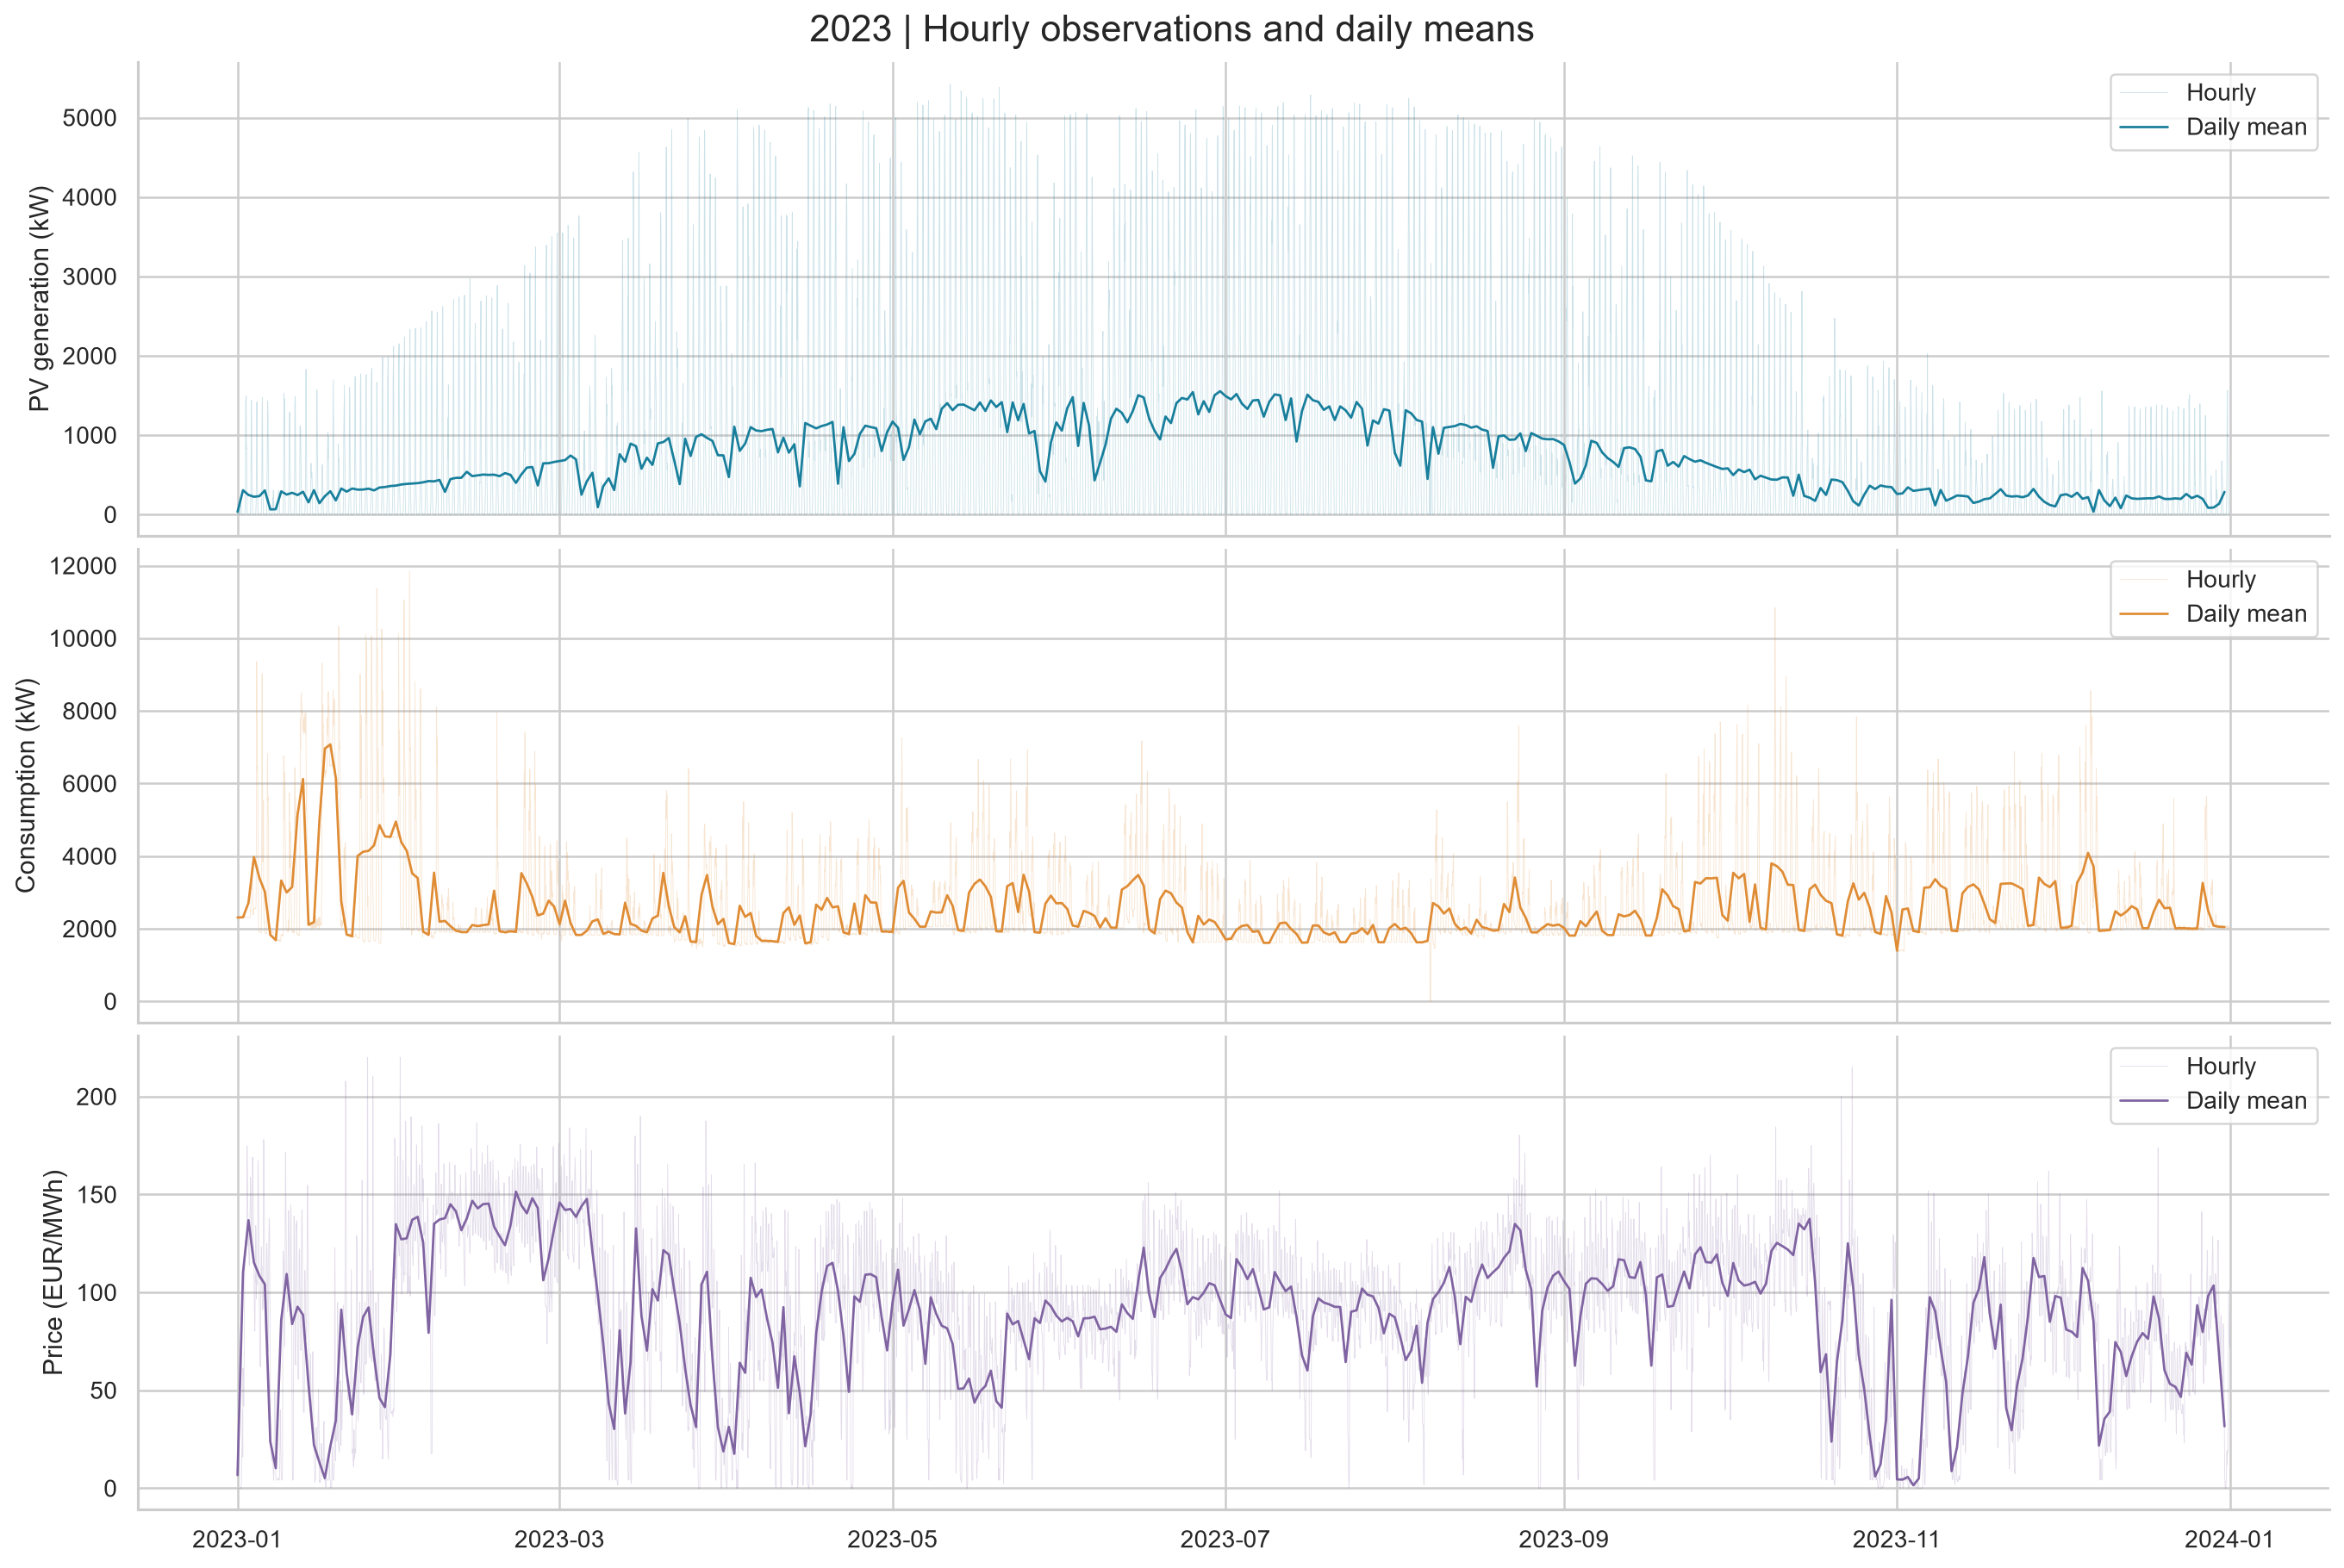
\includegraphics[width=0.95\linewidth]{figures/01_time_series.png}
\caption{2023 hourly observations and daily means for PV generation, load demand, and electricity price.}
\label{fig:time_series}
\end{figure}

\begin{figure}[htbp]
\centering
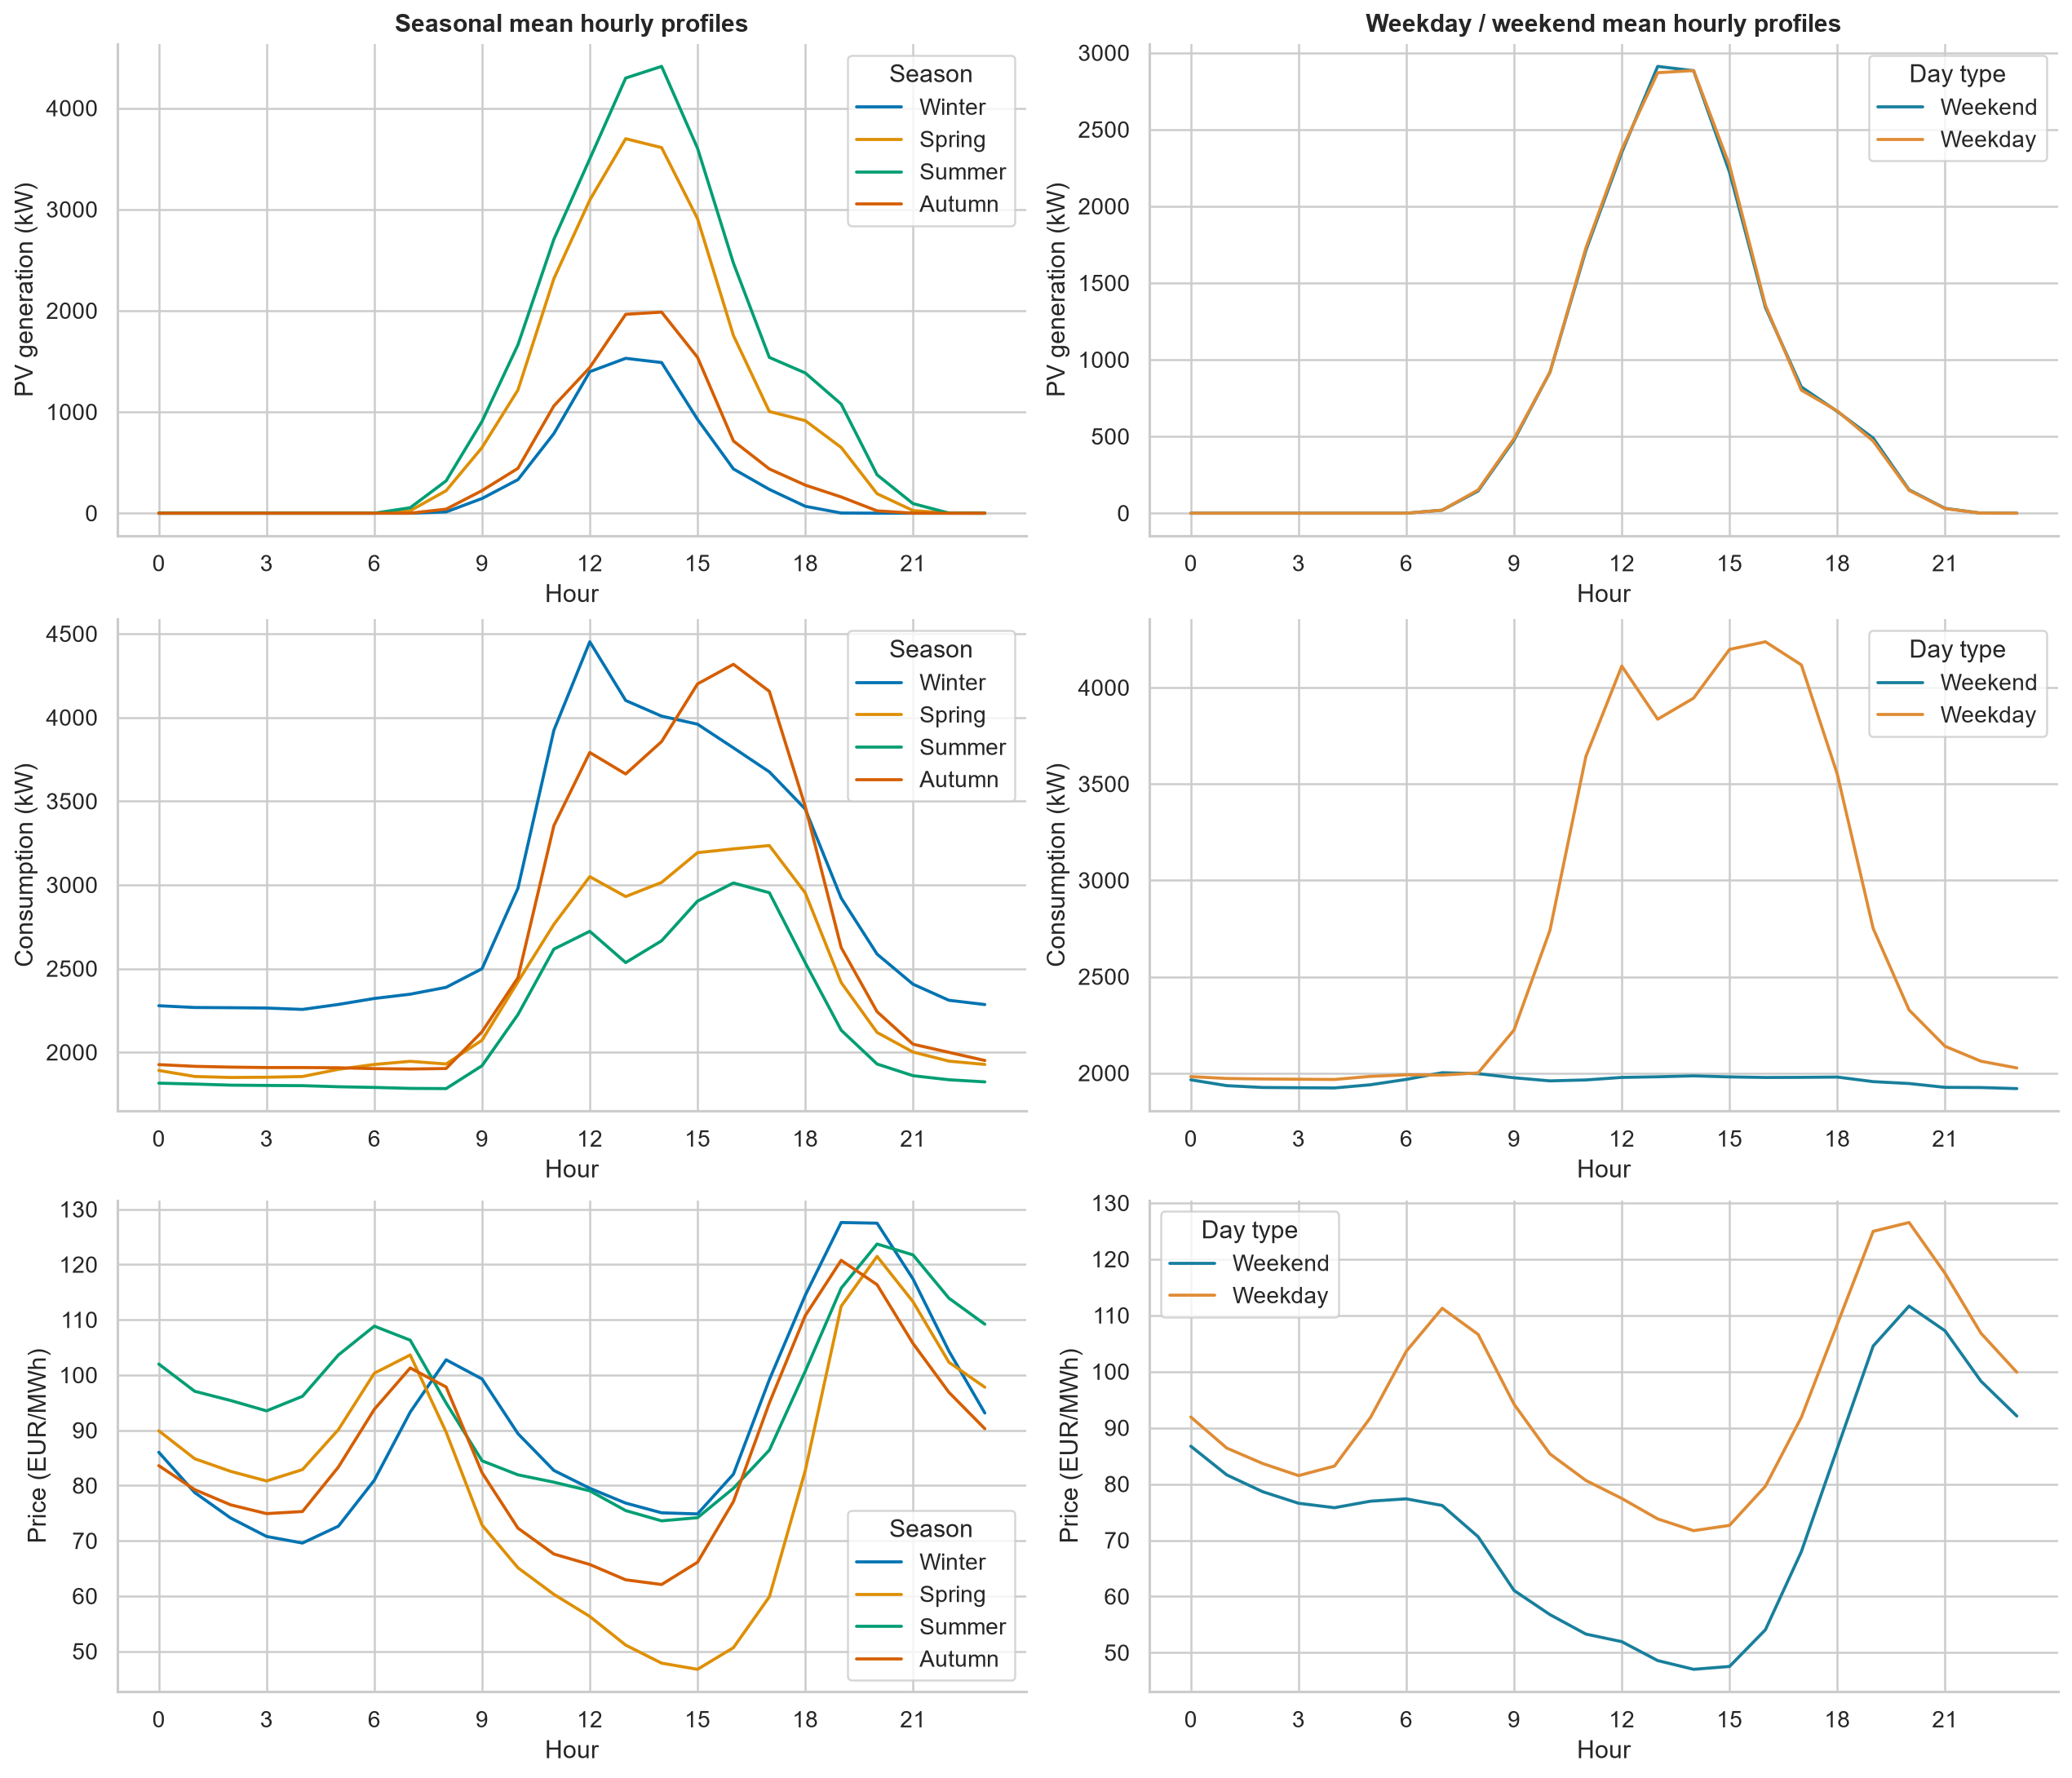
\includegraphics[width=0.95\linewidth]{figures/02_hourly_profiles.png}
\caption{Seasonal (left) and weekday/weekend (right) mean hourly profiles for PV, load, and price.}
\label{fig:hourly_profiles}
\end{figure}

\begin{table}[htbp]
\caption{Seasonal Hourly Means}
\label{tab:seasonal_means}
\begin{center}
\begin{tabular}{lccc}
\toprule
\textbf{Season} & \textbf{PV (kW)} & \textbf{Load (kW)} & \textbf{Price (EUR/MWh)} \\
\midrule
Winter & 306.6 & 2,919.2 & 90.5 \\
Spring & 928.3 & 2,344.4 & 81.1 \\
Summer & 1,183.6 & 2,160.7 & 95.8 \\
Autumn & 429.4 & 2,642.9 & 85.7 \\
\bottomrule
\end{tabular}
\end{center}
\end{table}

\textbf{Key observations:}
\begin{itemize}
    \item PV generation peaks at hour 14:00 (mean 2,884 kW) and is zero overnight. Summer mean PV (1,184 kW) is 3.9$\times$ winter mean (307 kW).
    \item Load peaks at hour 16:00 (mean 3,588 kW) with a minimum at 04:00 (1,954 kW). Winter mean load (2,919 kW) exceeds summer (2,161 kW) by 35\%.
    \item Price peaks at hour 20:00 (122.3 EUR/MWh) and reaches minimum at 14:00 (64.6 EUR/MWh), coinciding with peak PV.
    \item Weekday load exceeds weekend load by 780 kW on average (2,739 vs 1,958 kW), with a pronounced daytime ramp on weekdays absent on weekends. Weekend prices are 19.3 EUR/MWh lower on average.
\end{itemize}

Daily energy ranges are wide: PV 798–37,278 kWh/day (mean 17,160), Load 33,573–169,821 kWh/day (mean 60,342), confirming that average-day profiles do not capture extremes.

\begin{figure}[htbp]
\centering
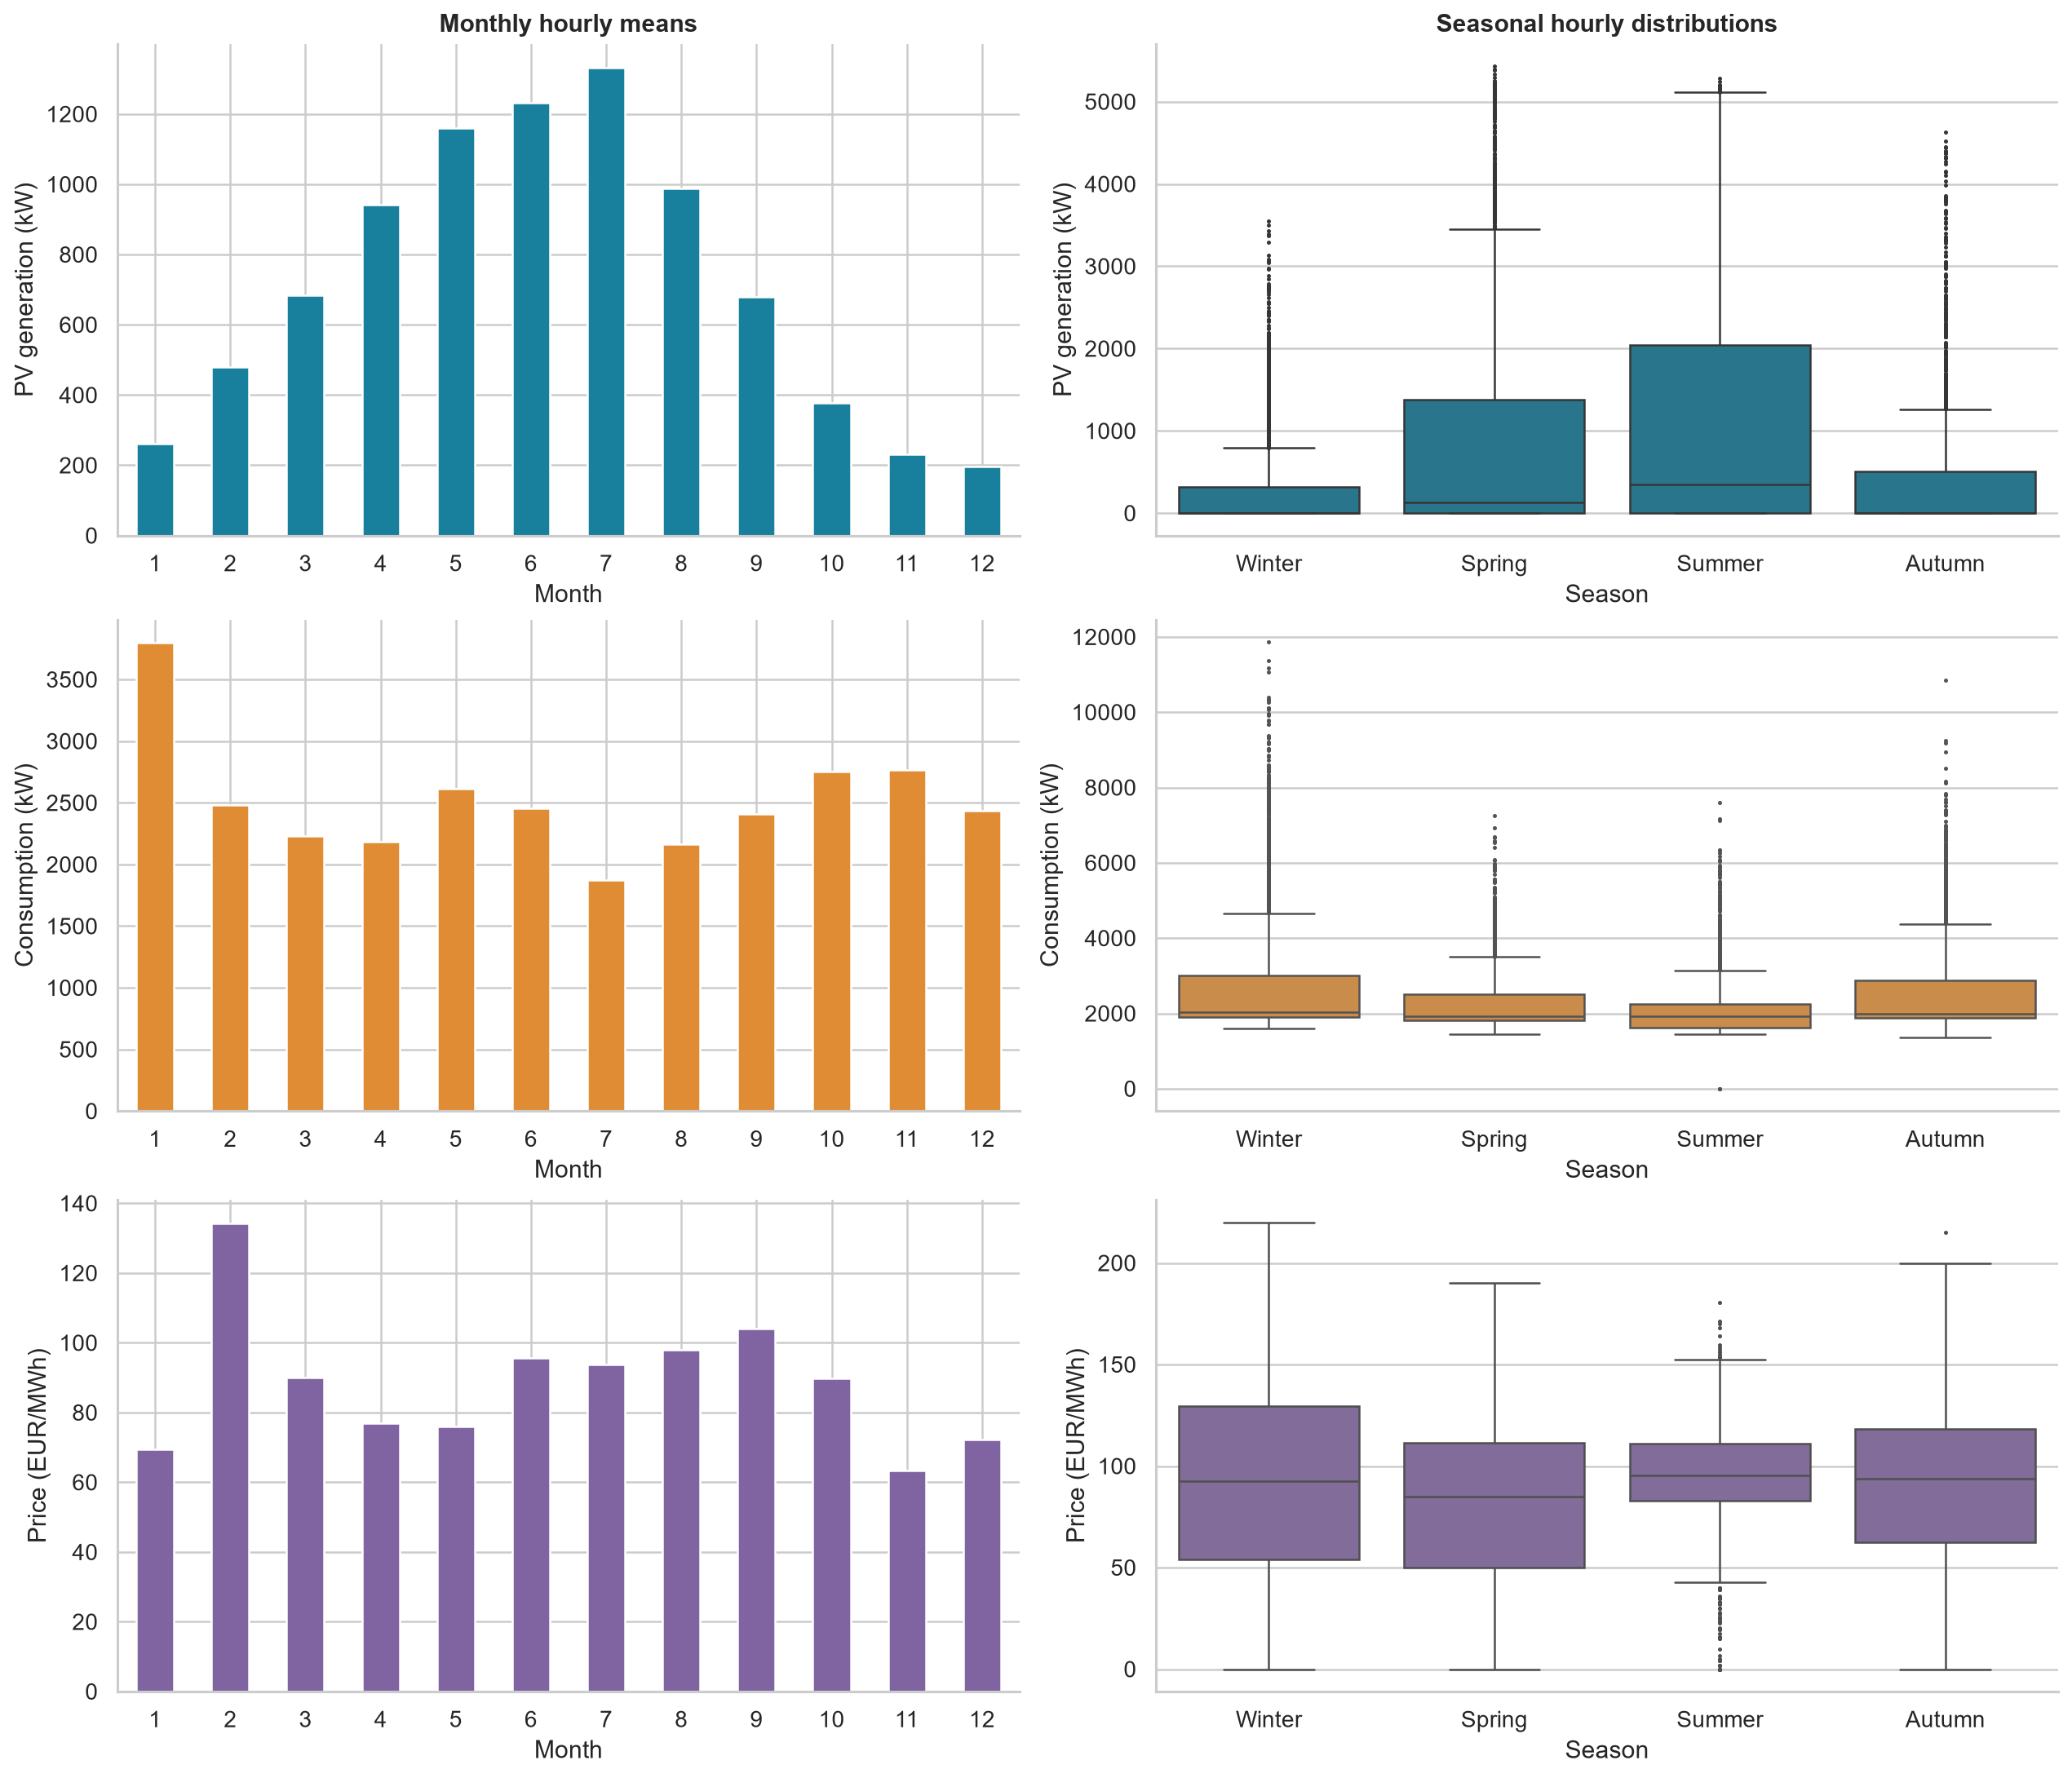
\includegraphics[width=0.95\linewidth]{figures/03_monthly_seasonal.png}
\caption{Monthly hourly means (left) and seasonal hourly distributions (right) for PV, load, and price.}
\label{fig:monthly_seasonal}
\end{figure}

\subsection{Correlation Structure and Aggregation Effects}
\label{sec:correlations}

Table~\ref{tab:correlation_comparison} shows Pearson and Spearman correlations at hourly and daily resolutions.

\begin{table}[htbp]
\caption{Correlation Comparison Across Time Scales}
\label{tab:correlation_comparison}
\begin{center}
\begin{tabular}{lccccc}
\toprule
\textbf{Pair} & \textbf{Hourly} & \textbf{Daily} & \textbf{Daytime} & \textbf{Hourly} & \textbf{Daily} \\
& \textbf{Pearson} & \textbf{Pearson} & \textbf{Pearson} & \textbf{Spearman} & \textbf{Spearman} \\
\midrule
PV / Load & +0.245 & -0.292 & +0.086 & +0.395 & -0.272 \\
PV / Price & -0.225 & +0.128 & -0.271 & -0.213 & +0.127 \\
Load / Price & -0.067 & +0.030 & -0.021 & -0.039 & +0.188 \\
\bottomrule
\end{tabular}
\end{center}
\end{table}

\textbf{Critical findings:}
\begin{enumerate}
    \item \textbf{Sign reversal under aggregation}: PV–Load correlation reverses from positive hourly (+0.245) to negative daily ($-$0.292). PV–Price reverses from negative hourly ($-$0.225) to positive daily (+0.128). This demonstrates that aggregation fundamentally changes the observed relationship—hourly correlations mix diurnal cycles, while daily correlations compare whole-day weather and activity patterns.
    \item \textbf{Daytime subset weakens PV–Load link}: Restricting to PV $>$ 0 hours reduces PV–Load Pearson to +0.086, showing the all-hour positive correlation partly stems from coincident nighttime zeros.
    \item \textbf{Seasonal instability of PV–Price}: Hourly PV–Price Pearson varies dramatically by season: Winter +0.007, Spring $-$0.413, Summer $-$0.453, Autumn $-$0.130. The negative correlation (merit-order effect) is strong in spring/summer but absent in winter.
    \item \textbf{Load–Price near zero}: At both hourly and daily scales, load–price correlation is negligible (Pearson $\approx$ 0), suggesting price is not strongly driven by demand alone in this market.
\end{enumerate}

Figure~\ref{fig:correlation_heatmaps} and Figure~\ref{fig:seasonal_correlations} visualize these patterns.

\begin{figure}[htbp]
\centering
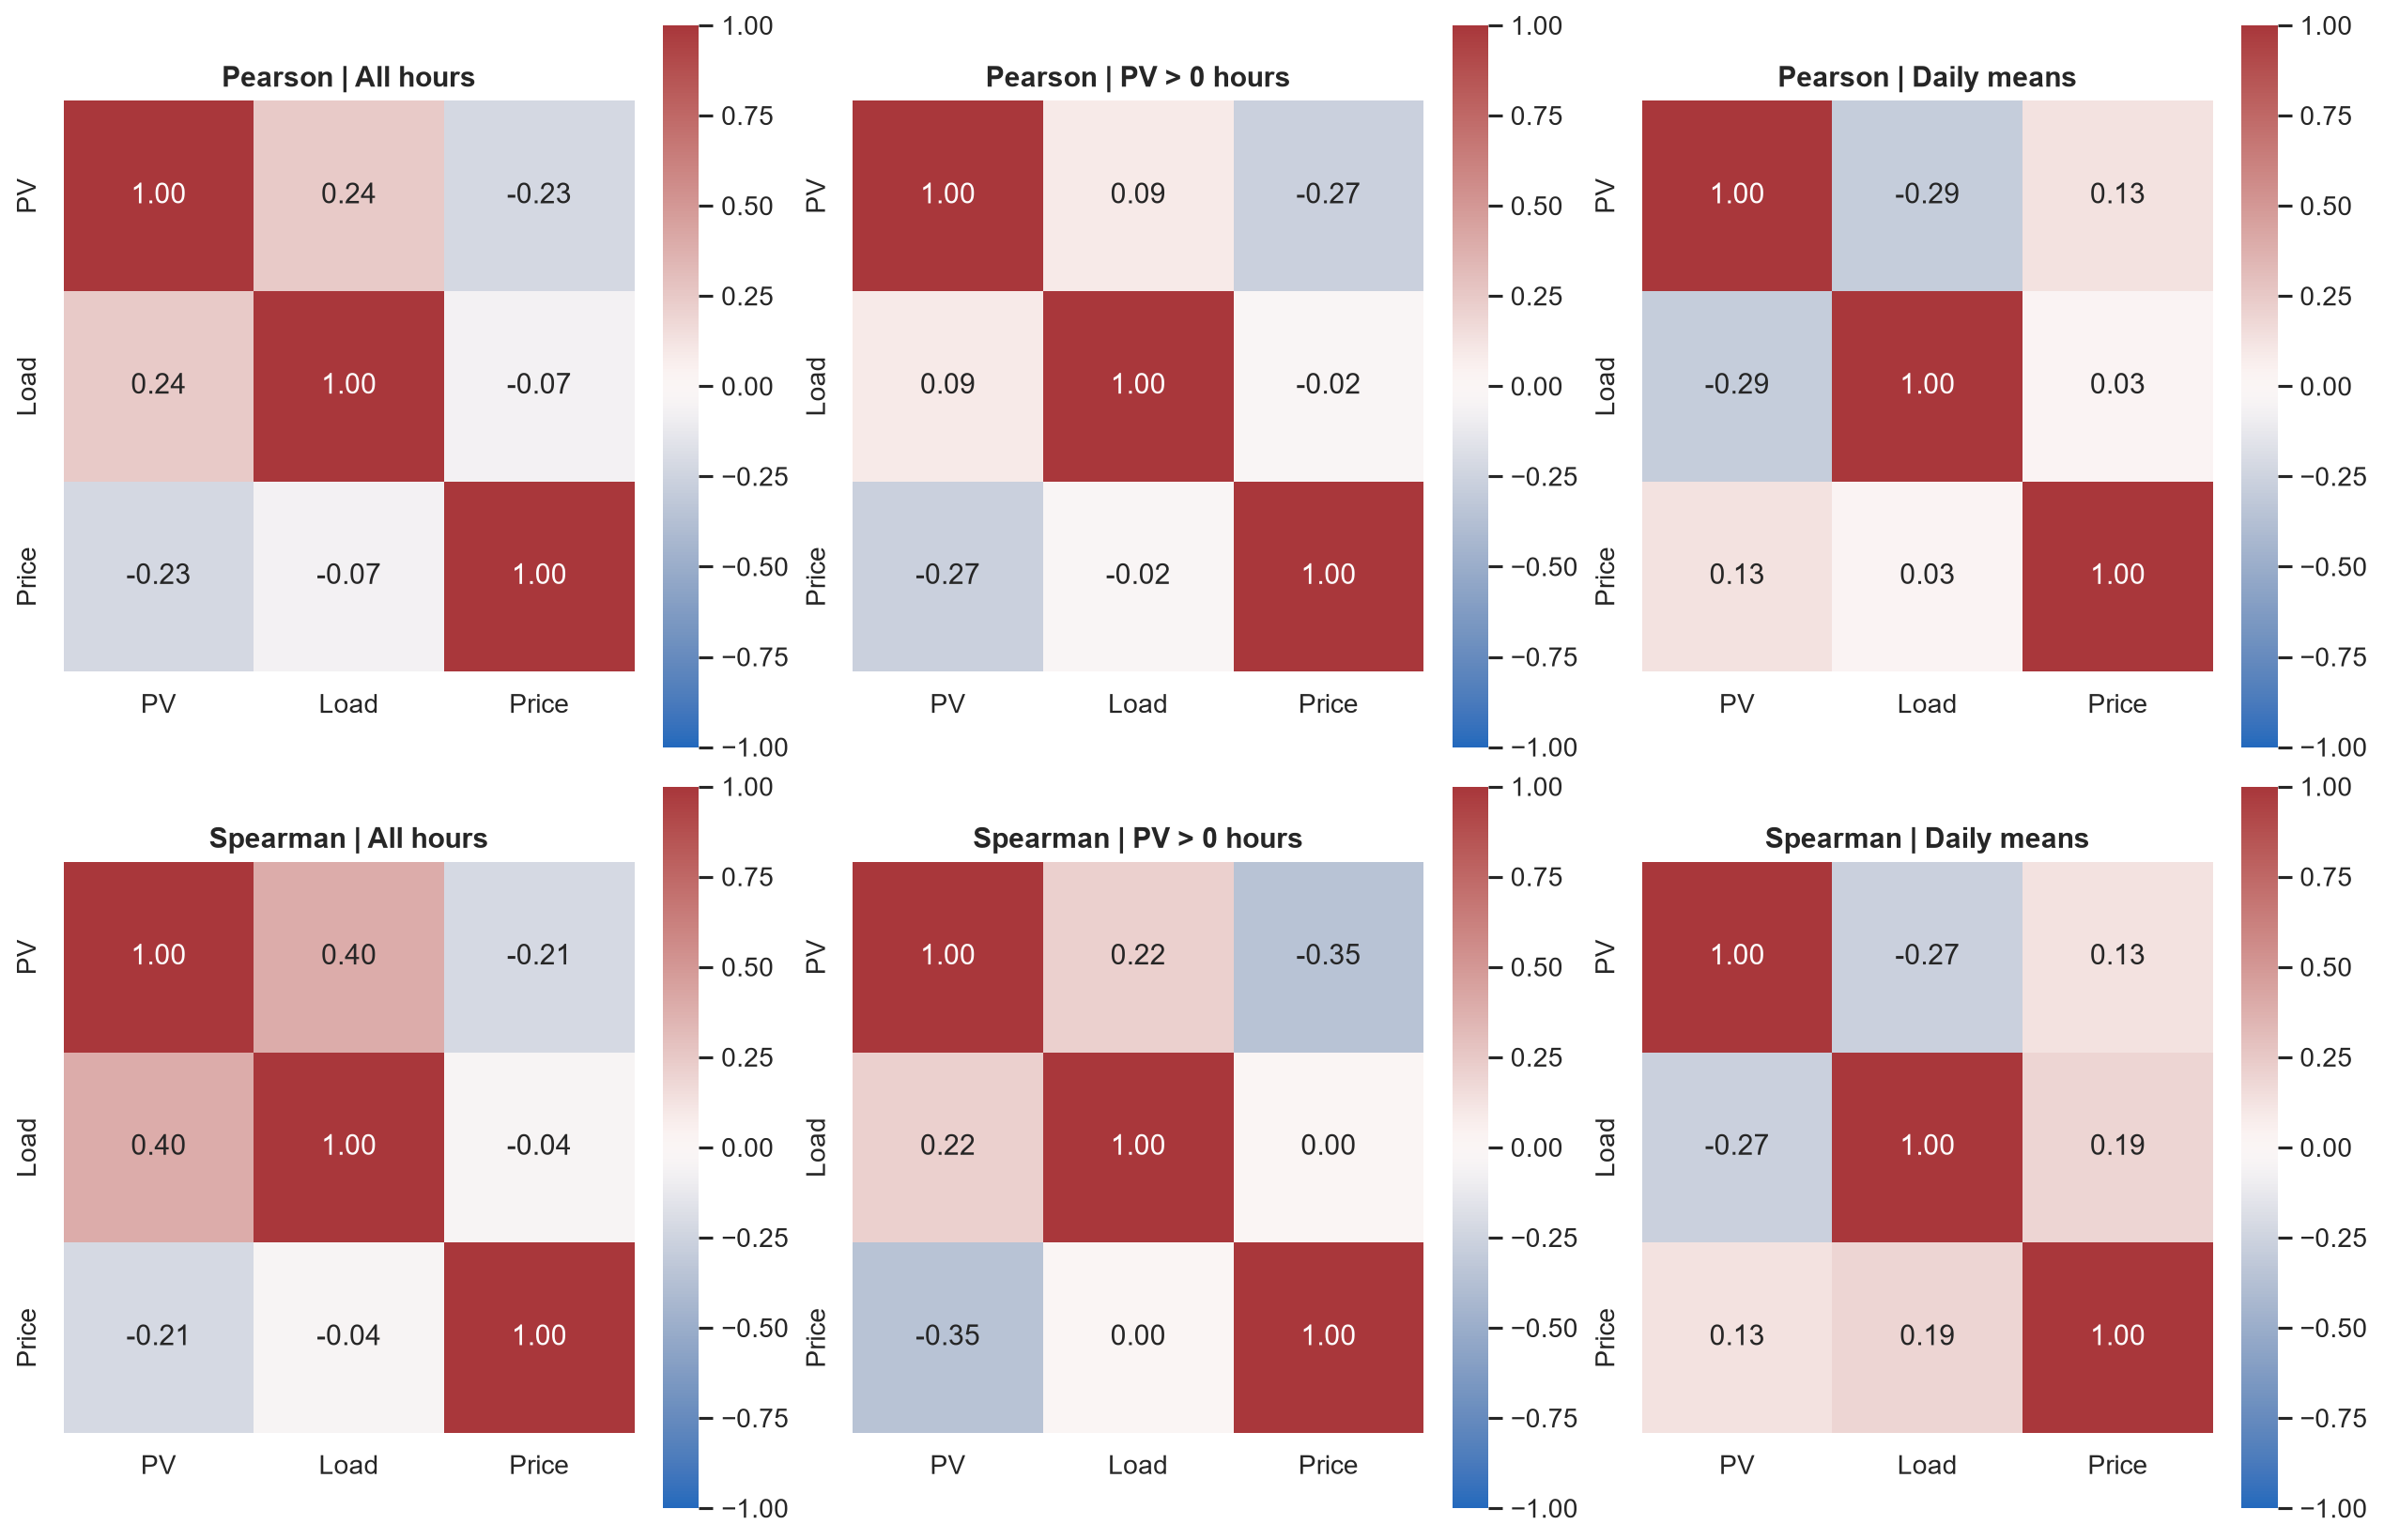
\includegraphics[width=0.95\linewidth]{figures/05_correlation_heatmaps.png}
\caption{Pearson (top) and Spearman (bottom) correlation heatmaps for all hours, daytime hours, and daily means.}
\label{fig:correlation_heatmaps}
\end{figure}

\begin{figure}[htbp]
\centering
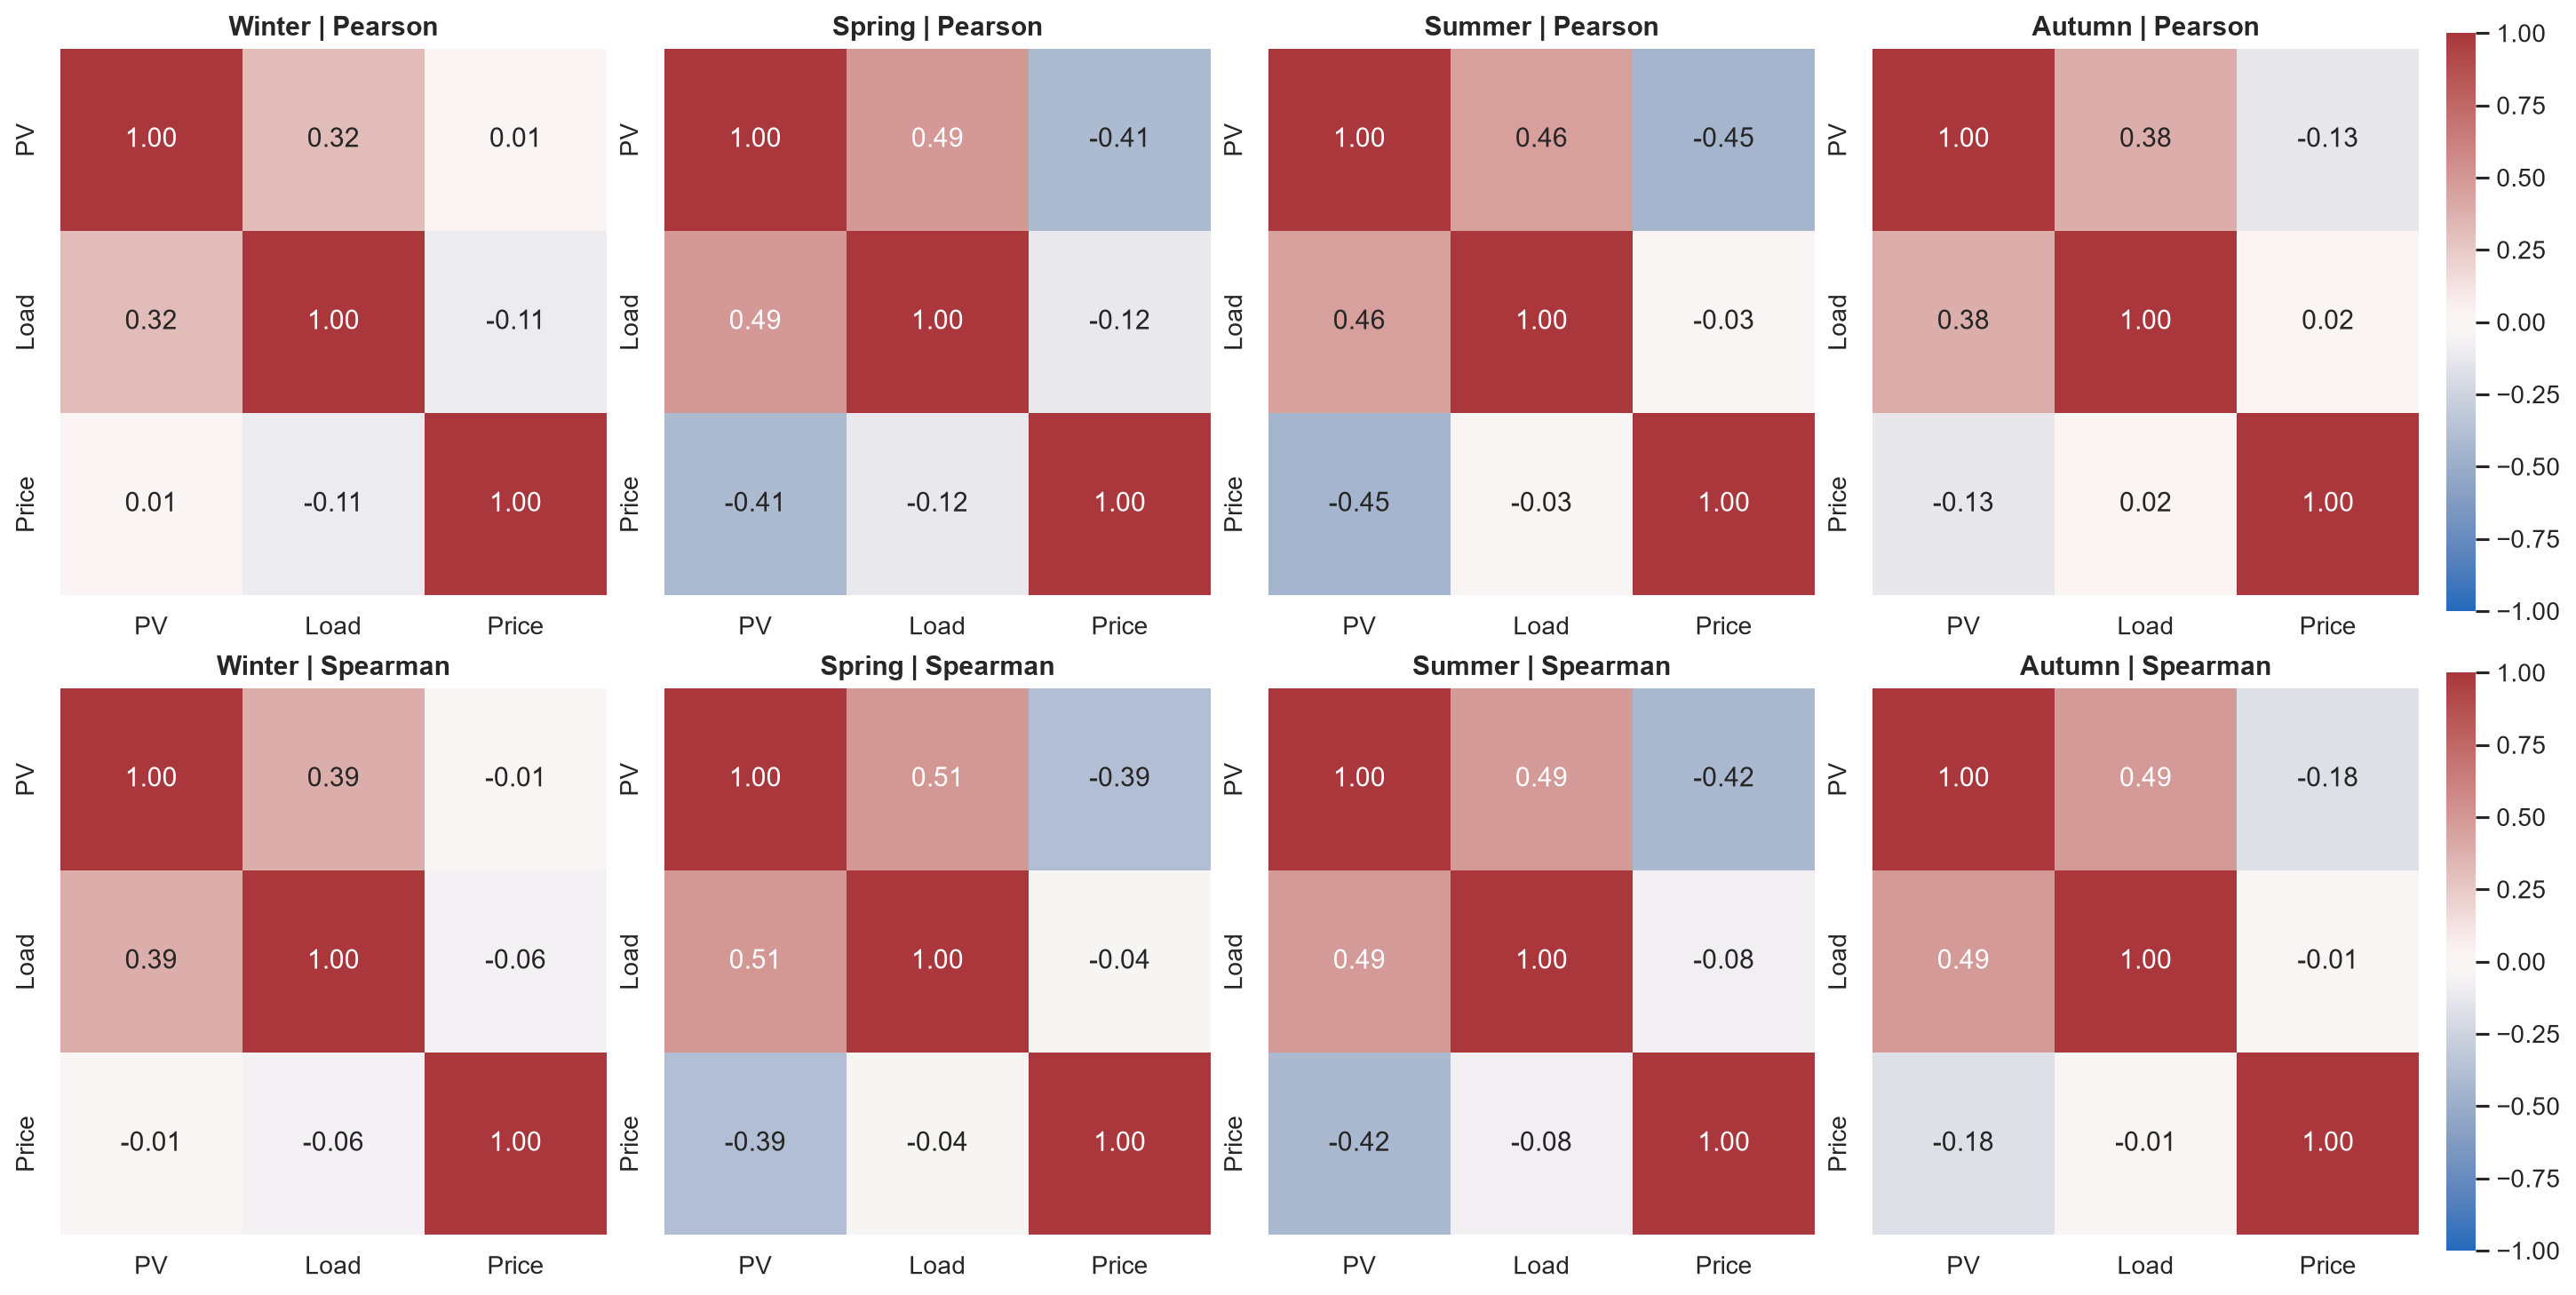
\includegraphics[width=0.95\linewidth]{figures/06_seasonal_correlations.png}
\caption{Seasonal hourly correlation heatmaps (Pearson top, Spearman bottom) for Winter, Spring, Summer, Autumn.}
\label{fig:seasonal_correlations}
\end{figure}

\begin{figure}[htbp]
\centering
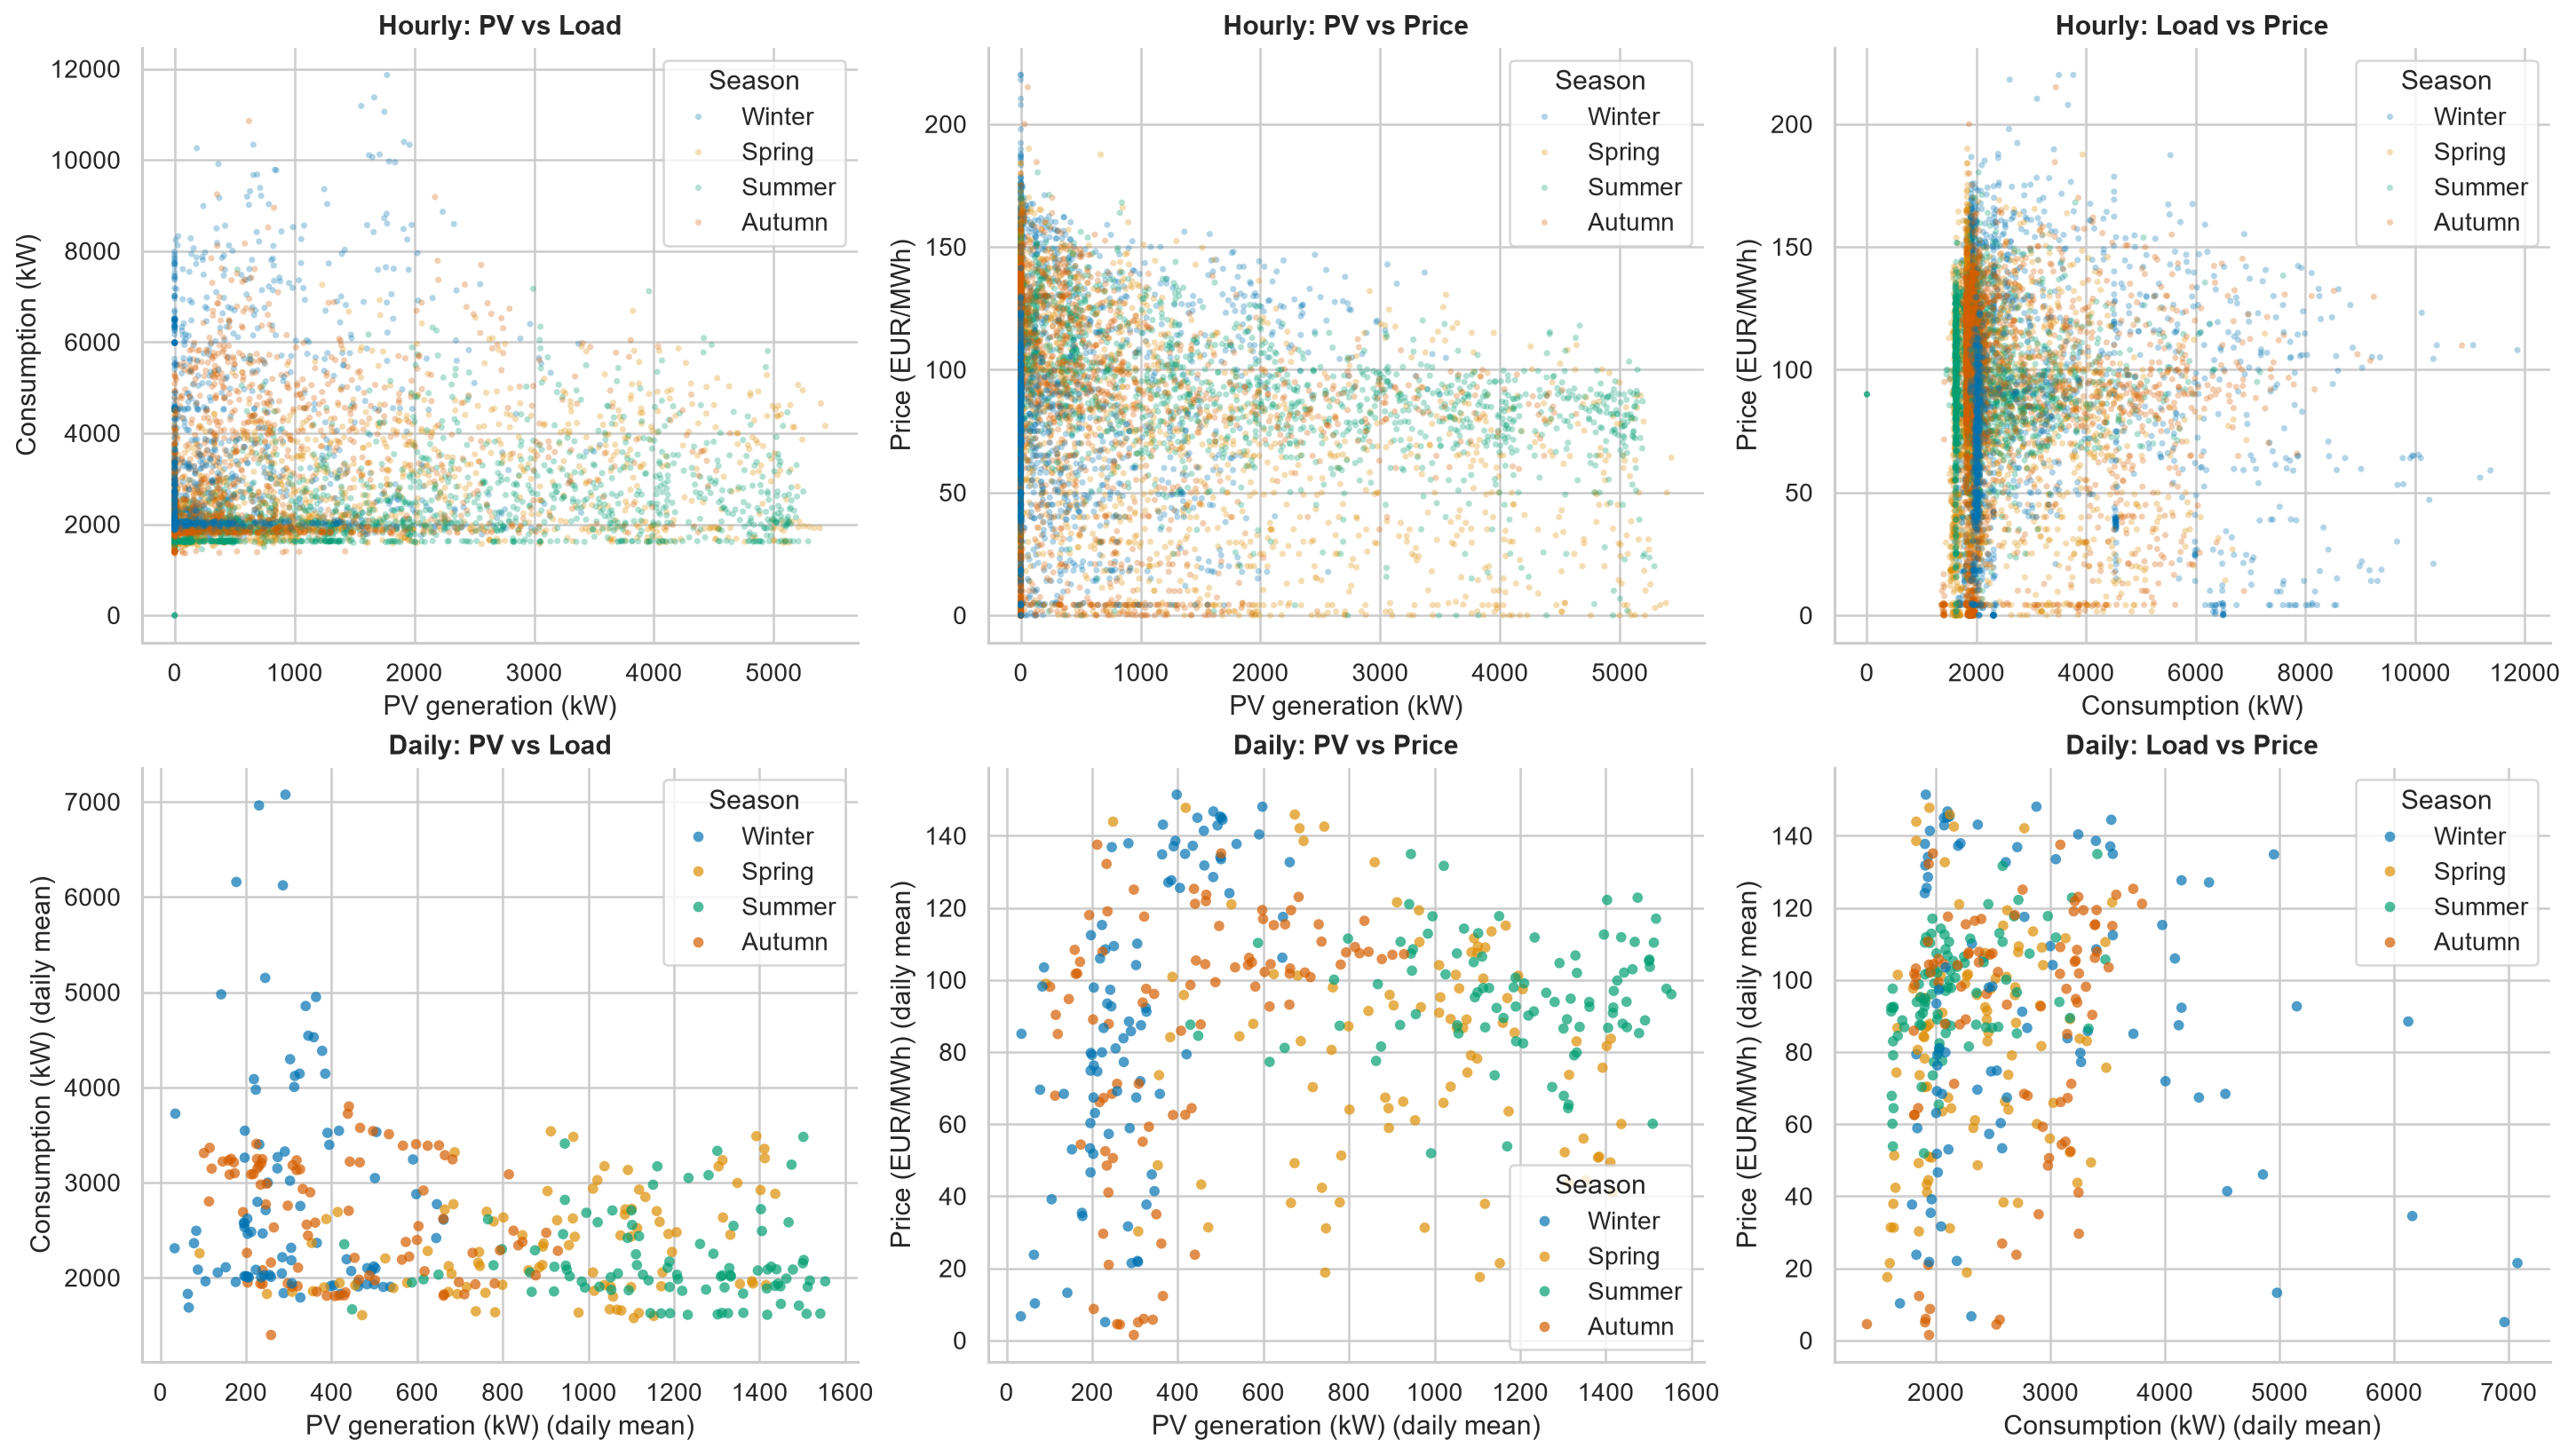
\includegraphics[width=0.95\linewidth]{figures/04_hourly_daily_scatter.png}
\caption{Hourly (top) and daily (bottom) scatter plots for PV vs Load, PV vs Price, and Load vs Price, colored by season.}
\label{fig:scatter}
\end{figure}

\subsection{Solar Surplus, Grid Deficit, and Economics}
\label{sec:surplus}

Annual totals: PV generation 6,263,310 kWh; Load demand 22,024,941 kWh. PV meets 28.4\% of annual energy demand.

\begin{itemize}
    \item \textbf{Surplus hours}: 770 hours (8.8\% of year) with PV $>$ Load, totaling 1,012,146 kWh surplus.
    \item \textbf{Coincident self-consumption}: 5,251,164 kWh (23.8\% of demand) consumed in the same hour as generation.
    \item \textbf{Grid deficit}: 16,773,777 kWh (76.2\% of demand) must be imported.
    \item \textbf{Peak demand}: Maximum 11,866 kW on 2023-02-01 12:00 (PV = 1,772 kW, Price = 107.98 EUR/MWh).
    \item \textbf{Peak-hour prices}: Mean price during top 5\% load hours (438 hours) is 78.8 EUR/MWh vs. 88.8 EUR/MWh otherwise—a modest discount during peak demand.
    \item \textbf{Deficit–Price correlation}: Pearson +0.083 (hourly), indicating higher deficit mildly associates with higher prices.
    \item \textbf{Surplus–Price correlation}: Pearson $-$0.165 (hourly), confirming lower prices during solar surplus.
\end{itemize}

Load-weighted average price (86.9 EUR/MWh) is below time-average (88.3 EUR/MWh), reflecting lower prices during high-demand hours. Illustrative energy-only cost: 1,914,053 EUR (gross load) vs. 1,518,663 EUR (deficit only)—excluding tariffs, taxes, network fees, and export revenue.

Figure~\ref{fig:energy_balance_price} illustrates these relationships.

\begin{figure}[htbp]
\centering
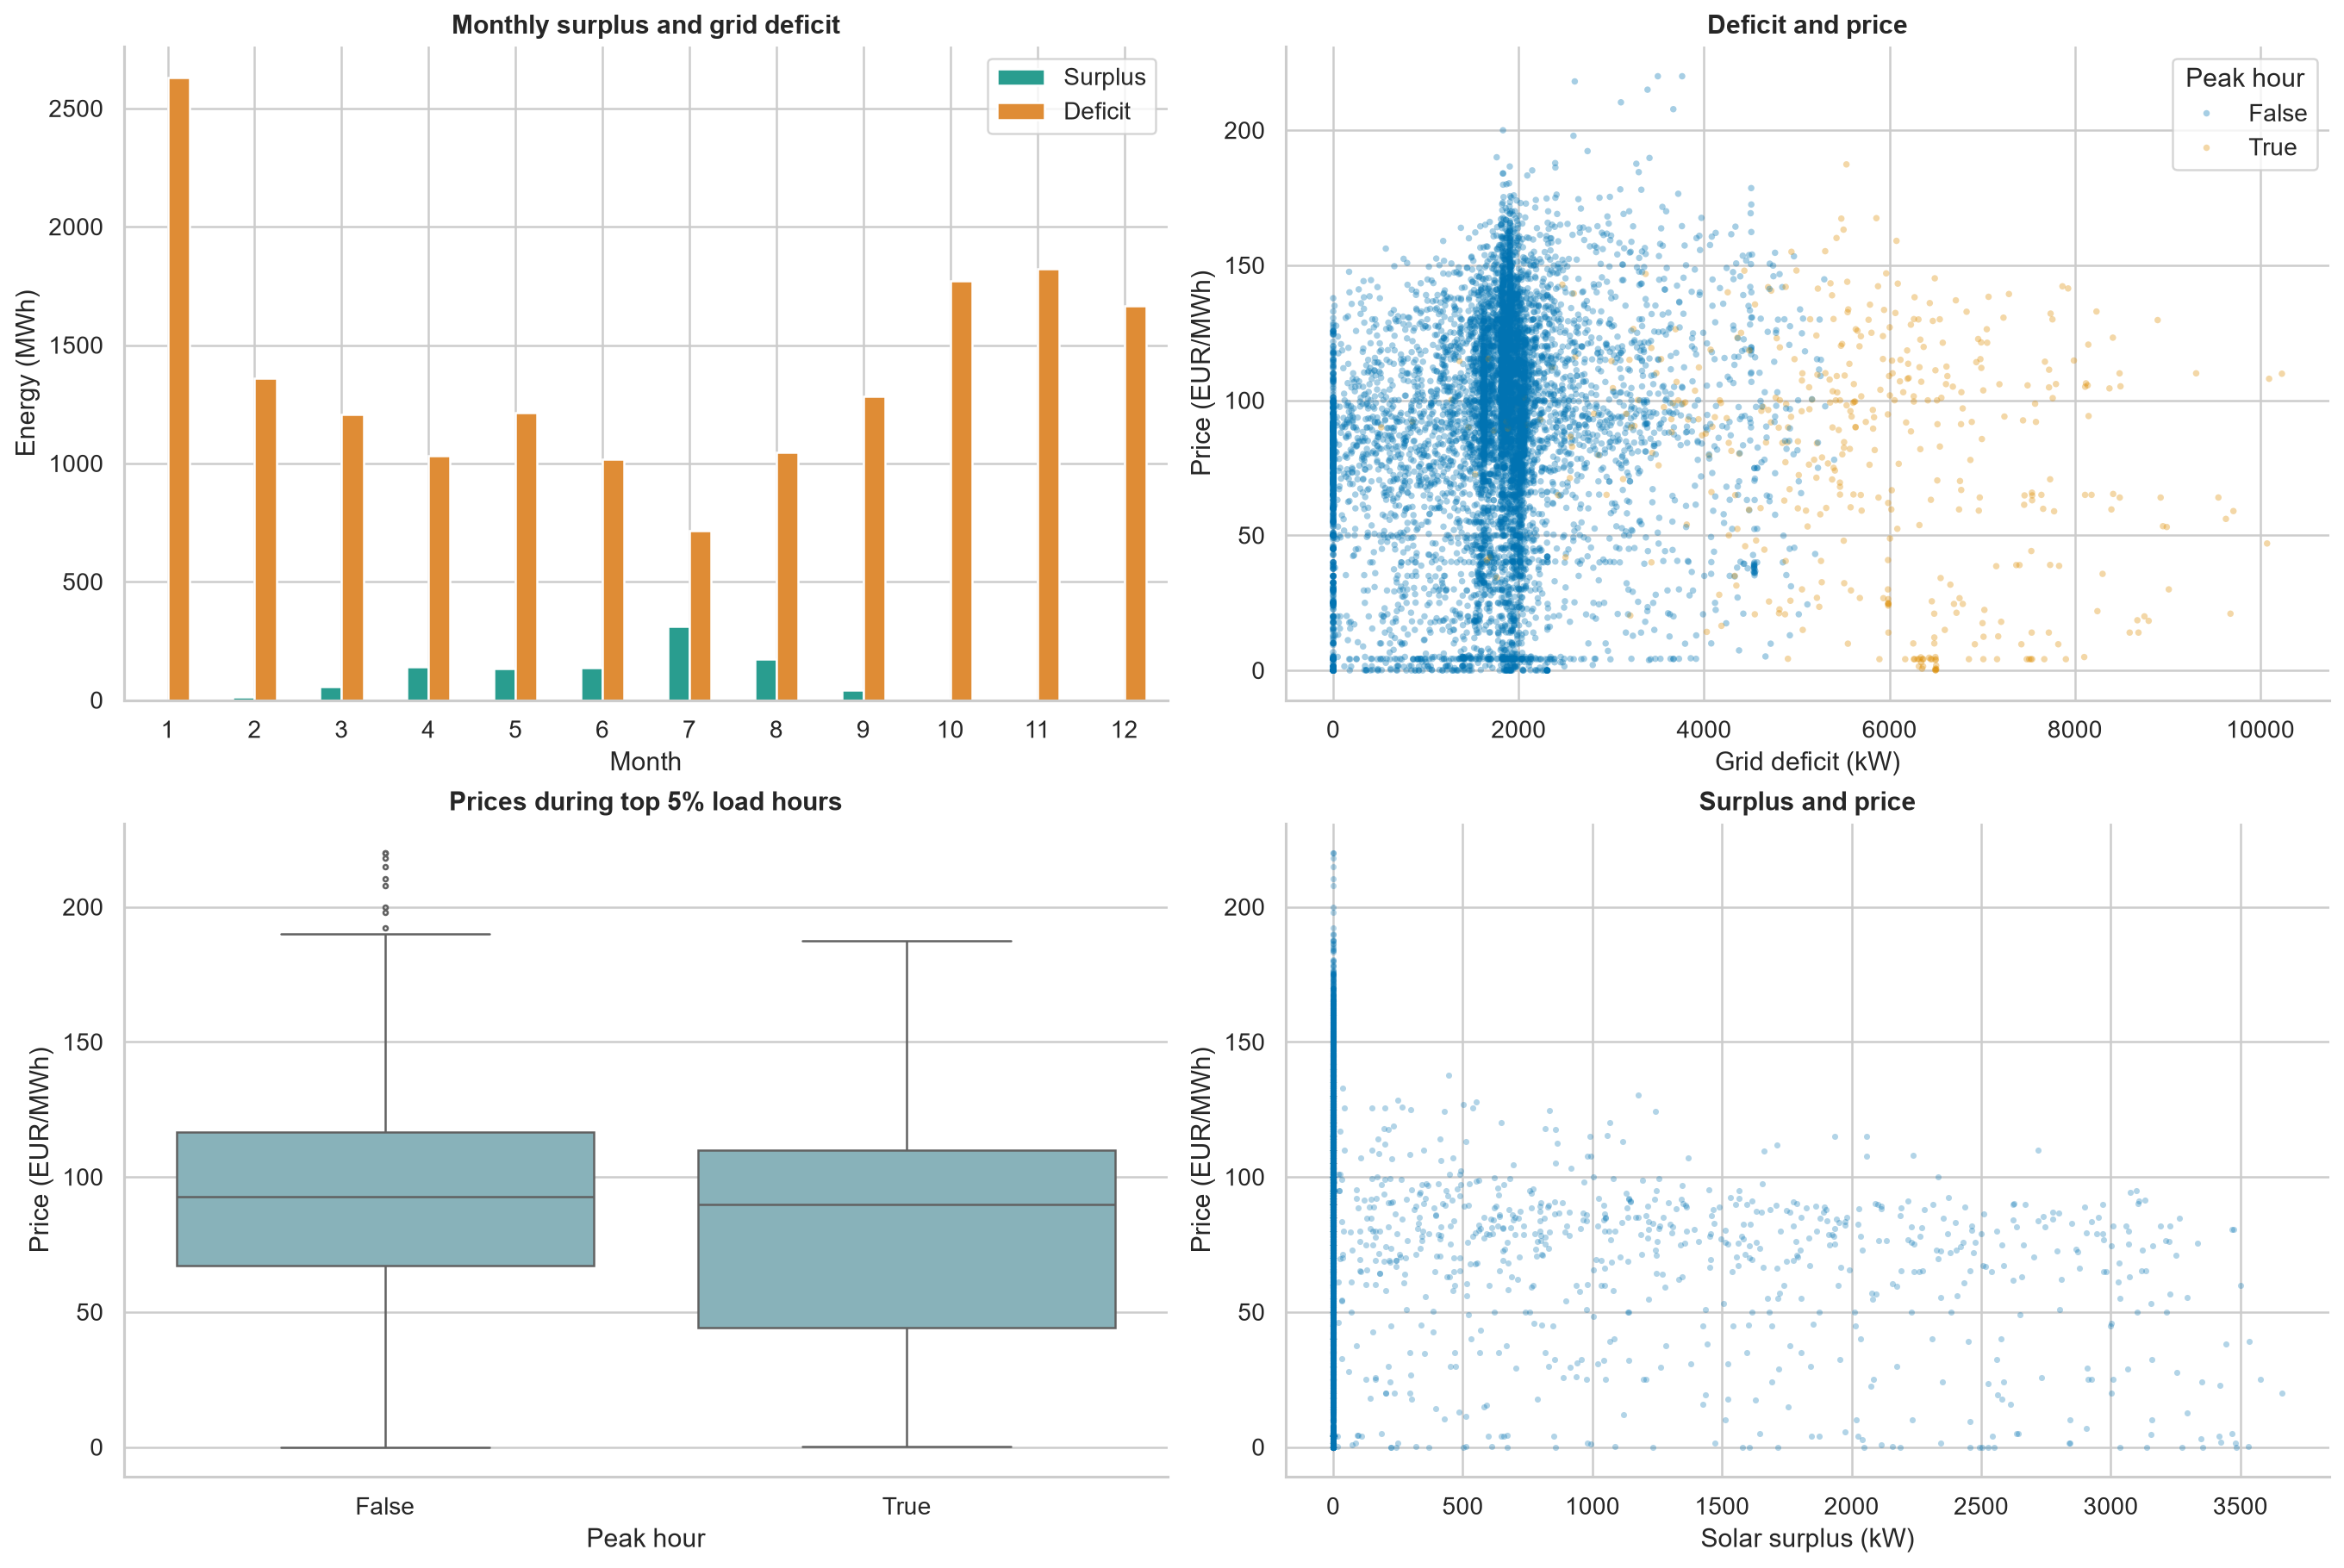
\includegraphics[width=0.95\linewidth]{figures/07_energy_balance_price.png}
\caption{Monthly surplus/deficit energy (top-left), deficit vs price (top-right), price during peak hours (bottom-left), surplus vs price (bottom-right).}
\label{fig:energy_balance_price}
\end{figure}

\subsection{Data Quality Observations}
\label{sec:quality}

\begin{figure}[htbp]
\centering
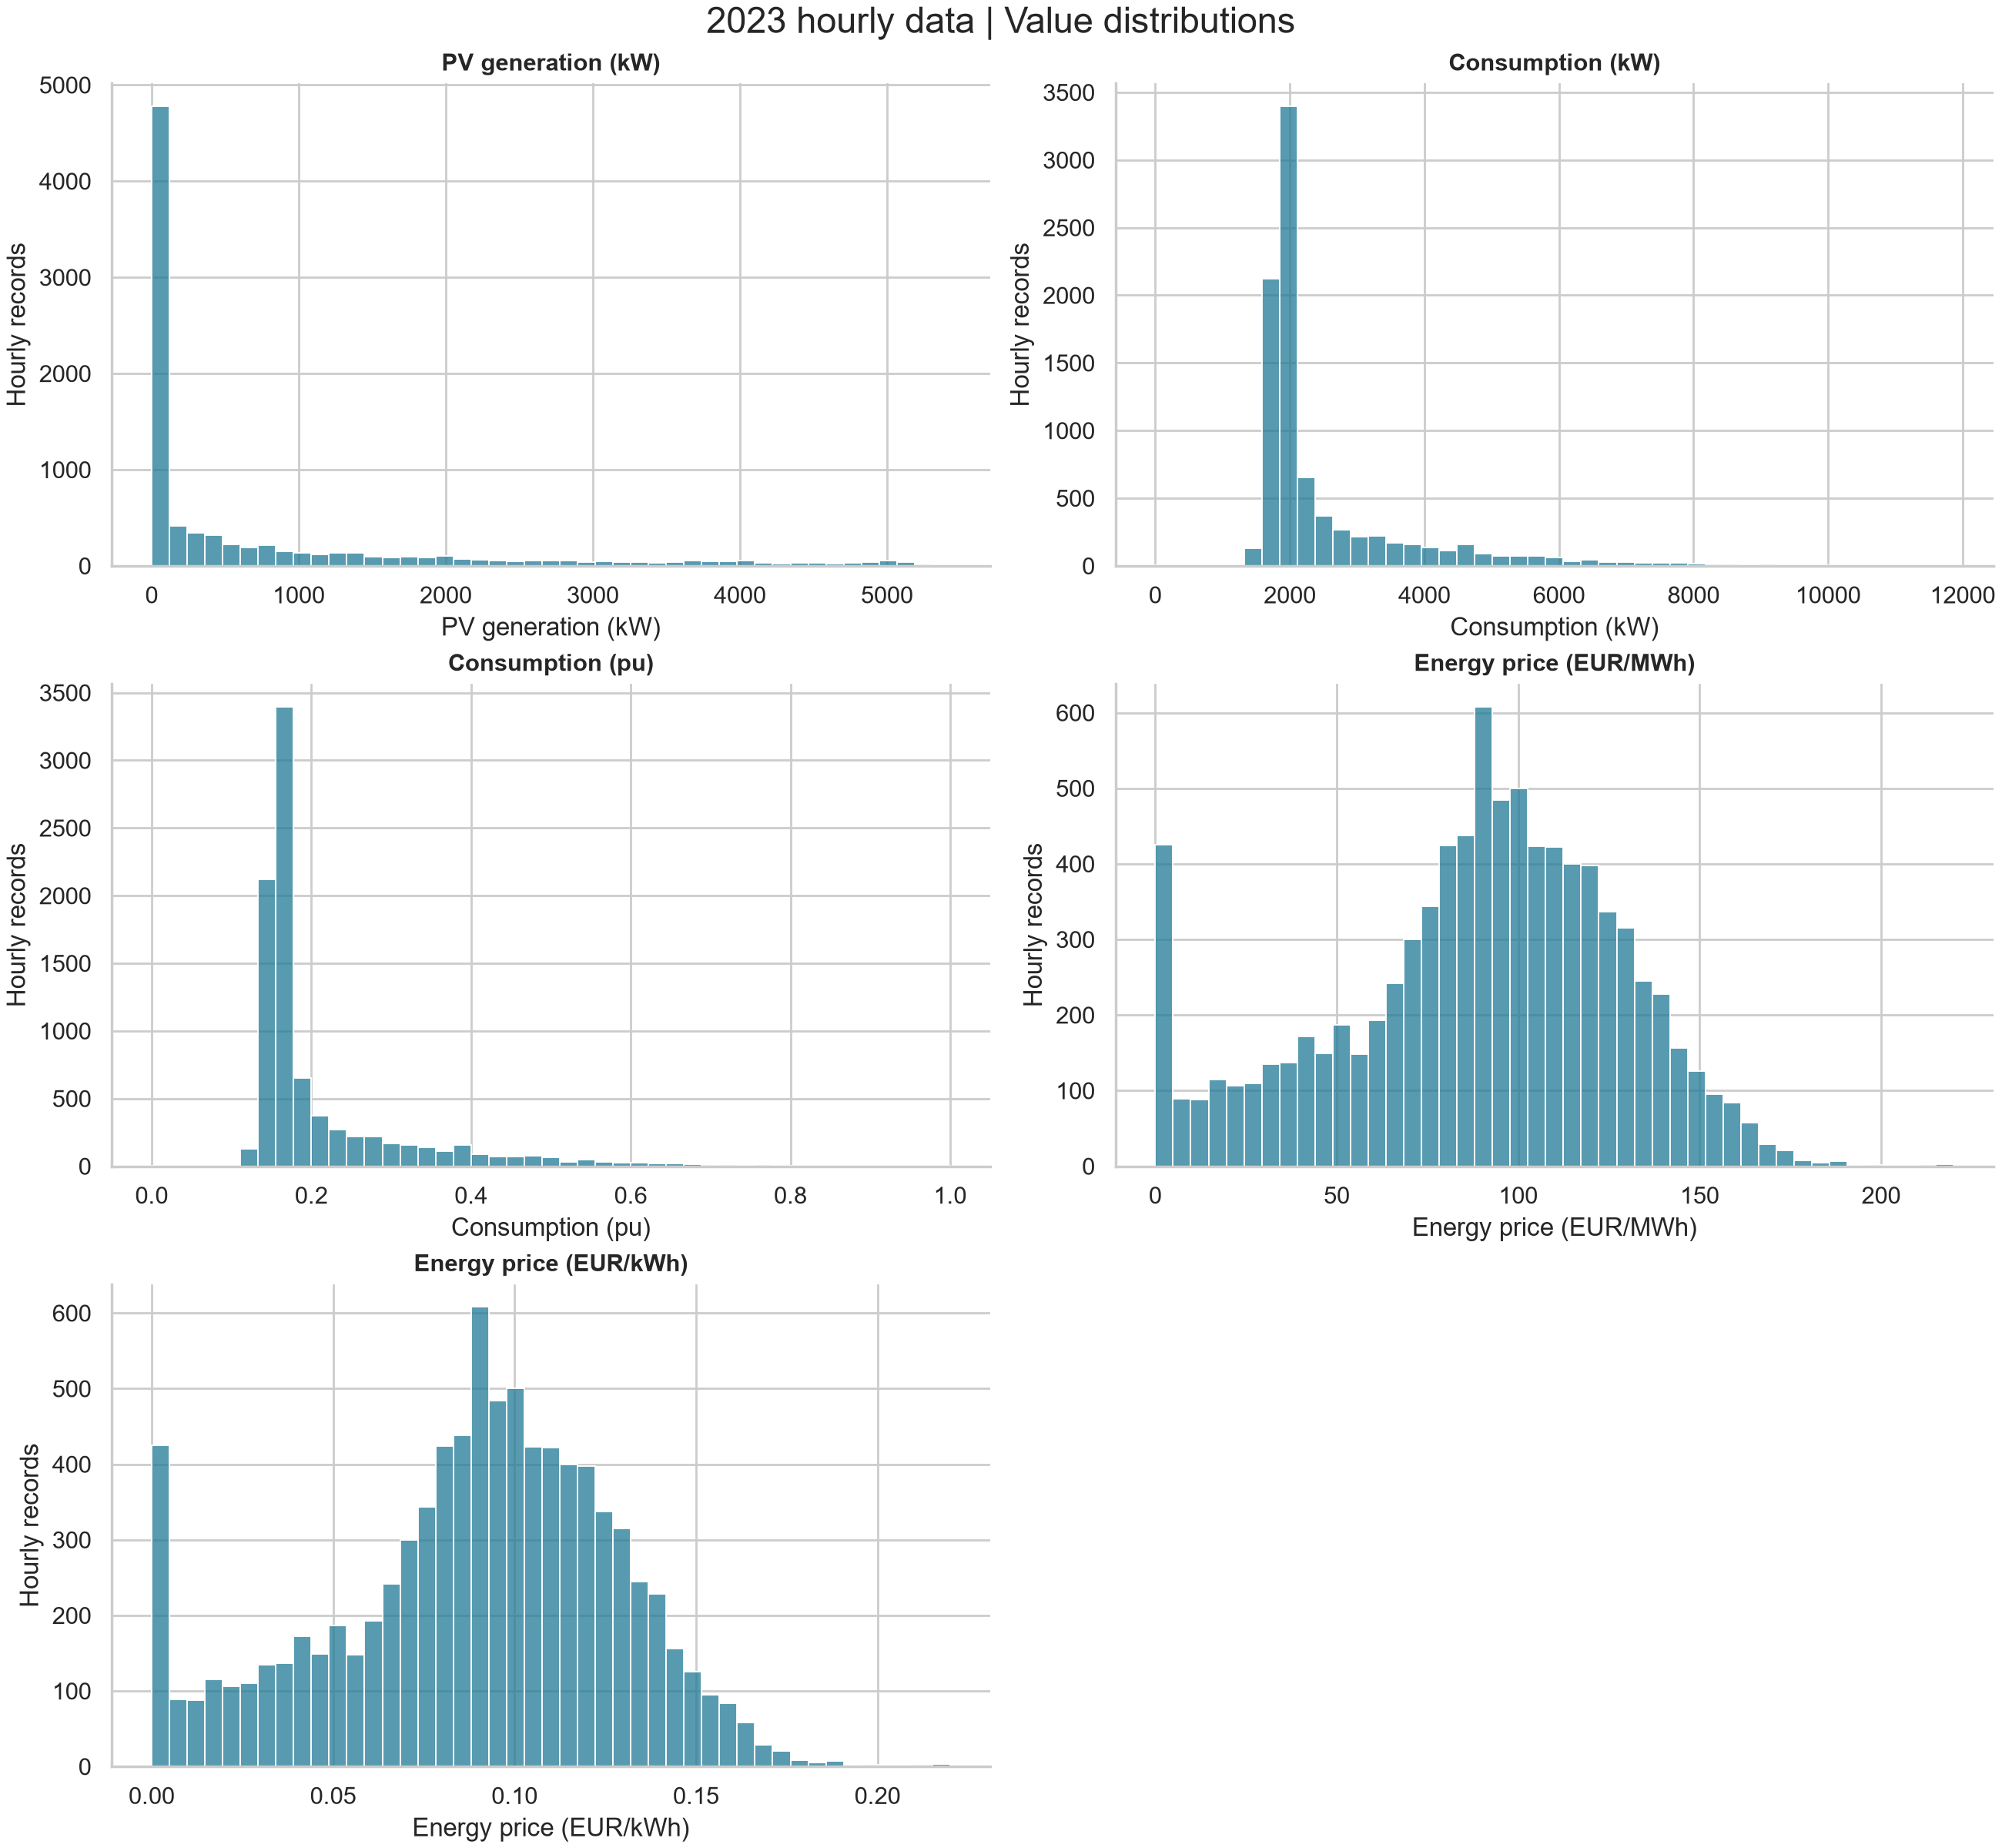
\includegraphics[width=0.95\linewidth]{figures/distributions.png}
\caption{Histograms of PV generation, load demand, and electricity price showing frequency distributions and skew.}
\label{fig:distributions}
\end{figure}

\begin{figure}[htbp]
\centering
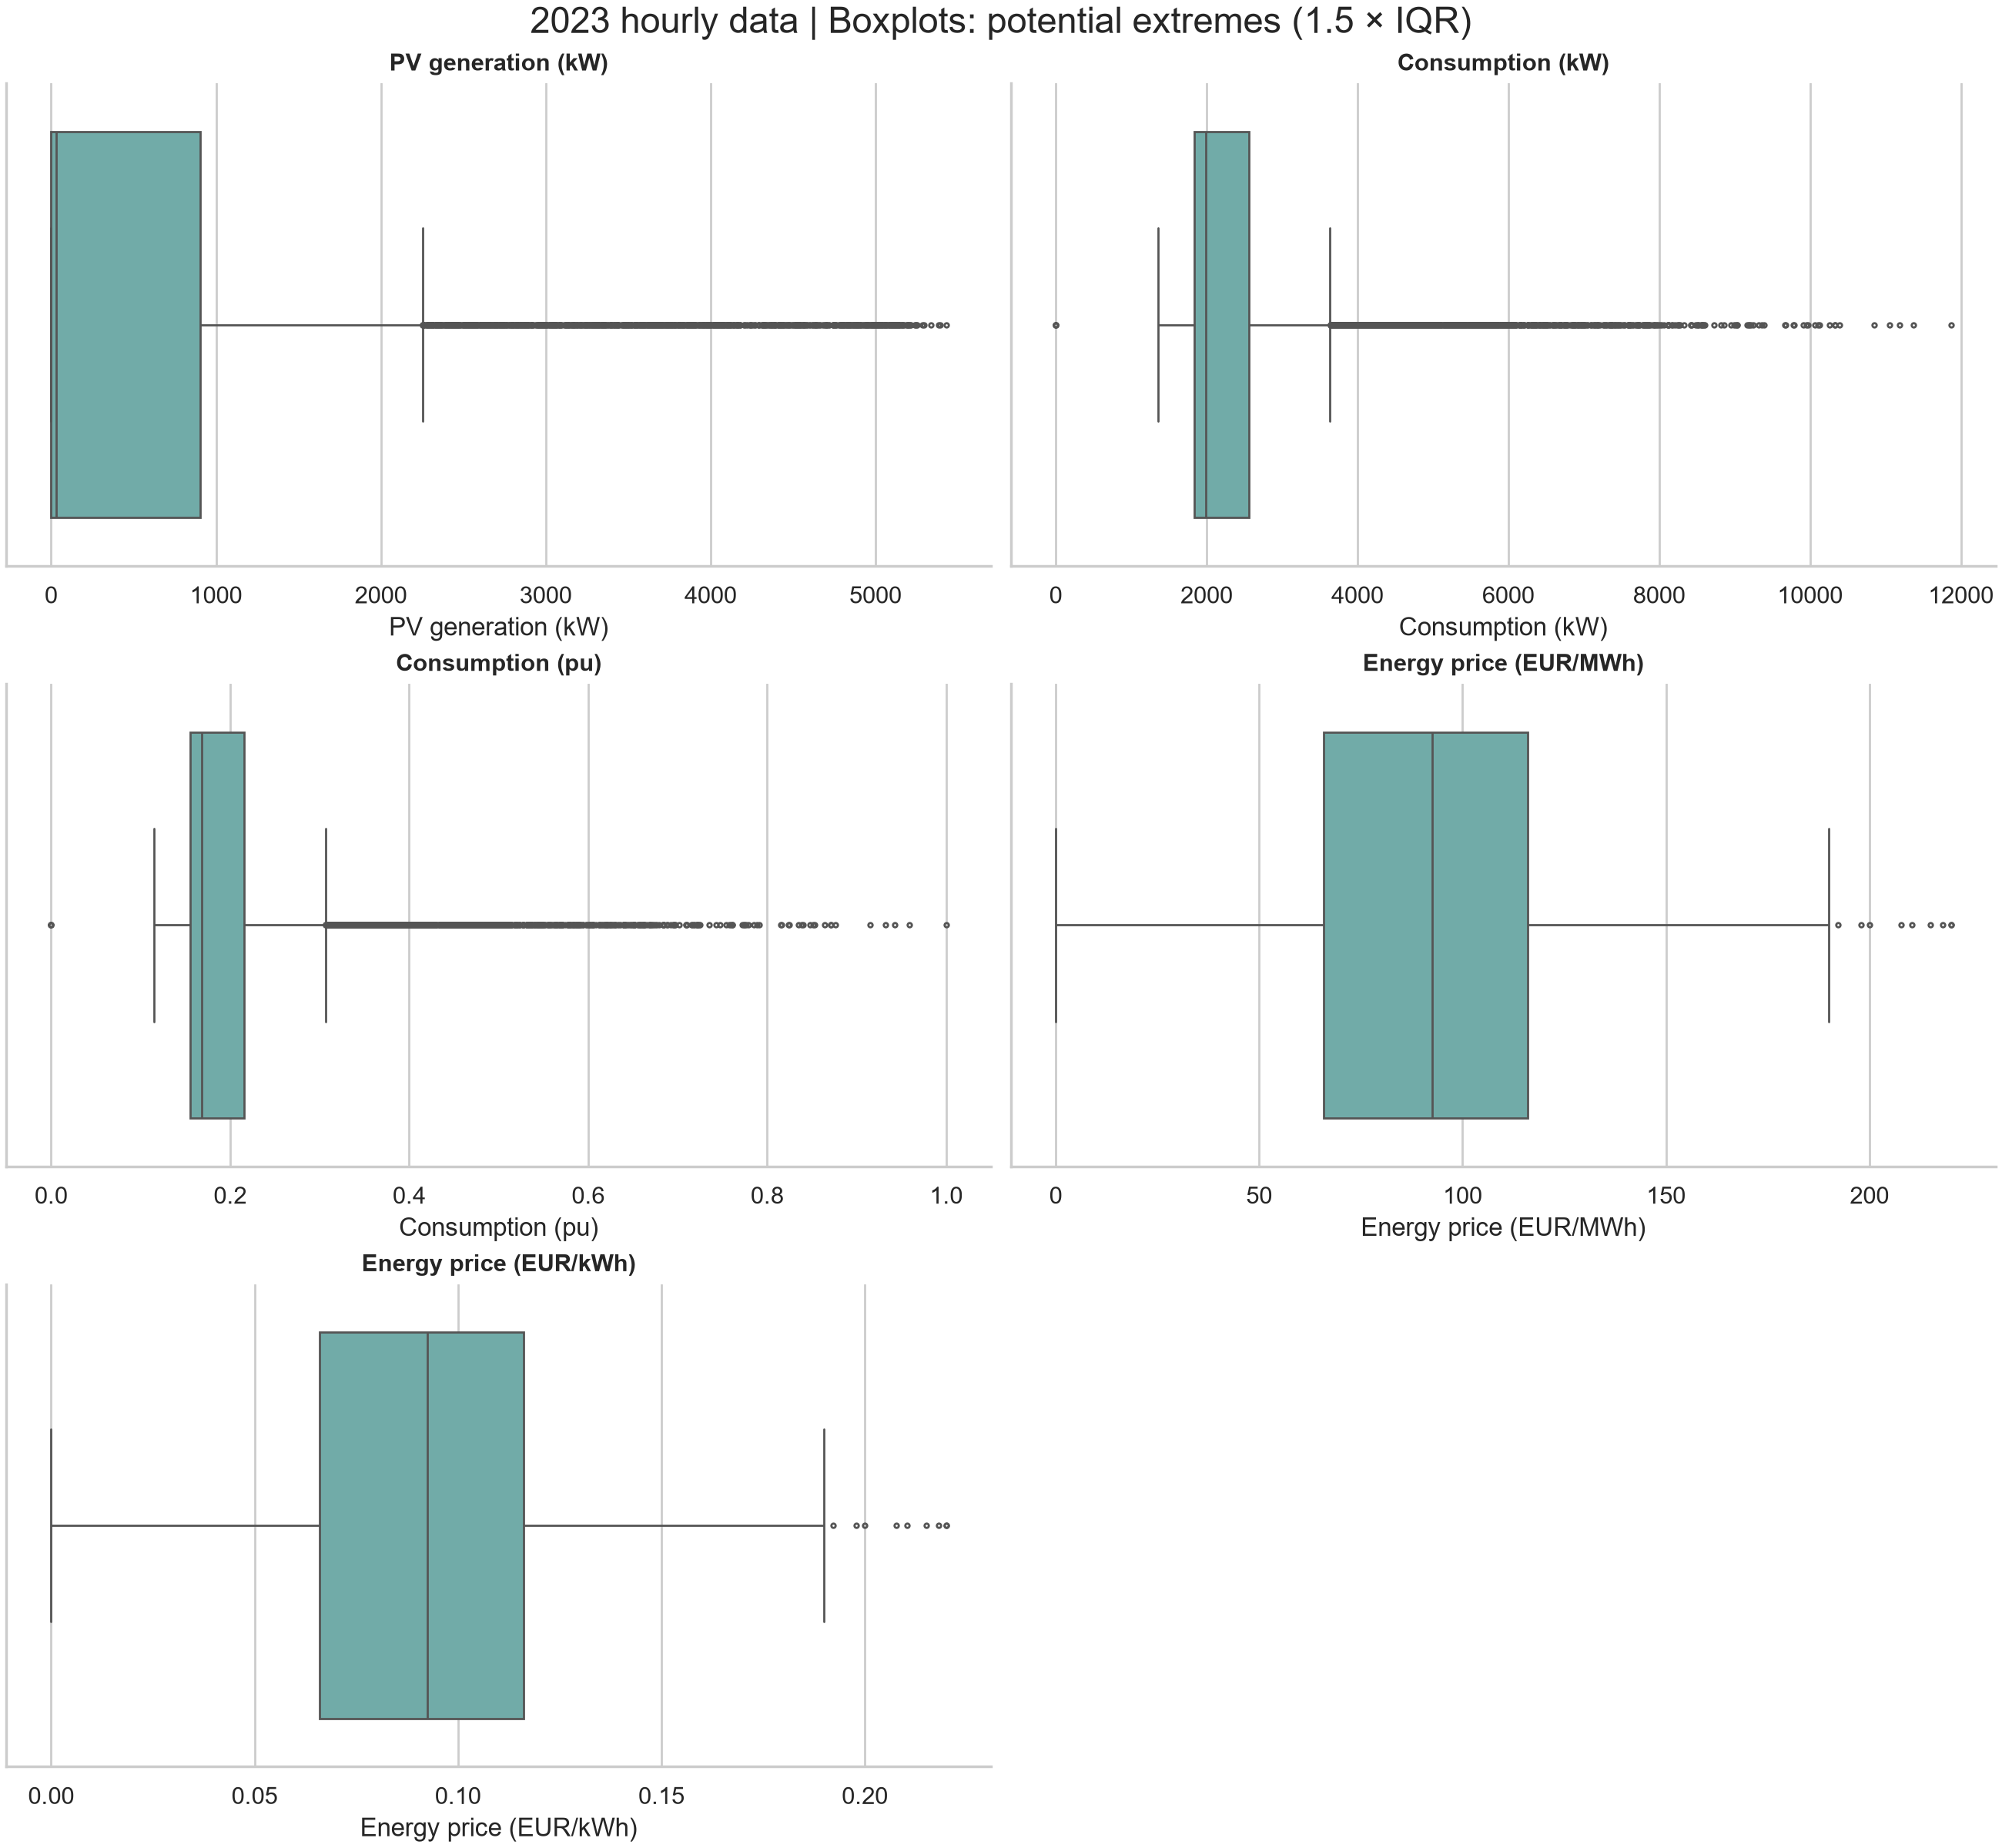
\includegraphics[width=0.95\linewidth]{figures/boxplots.png}
\caption{Boxplots of core variables with IQR-based outlier flags (dots).}
\label{fig:boxplots}
\end{figure}

\begin{figure}[htbp]
\centering
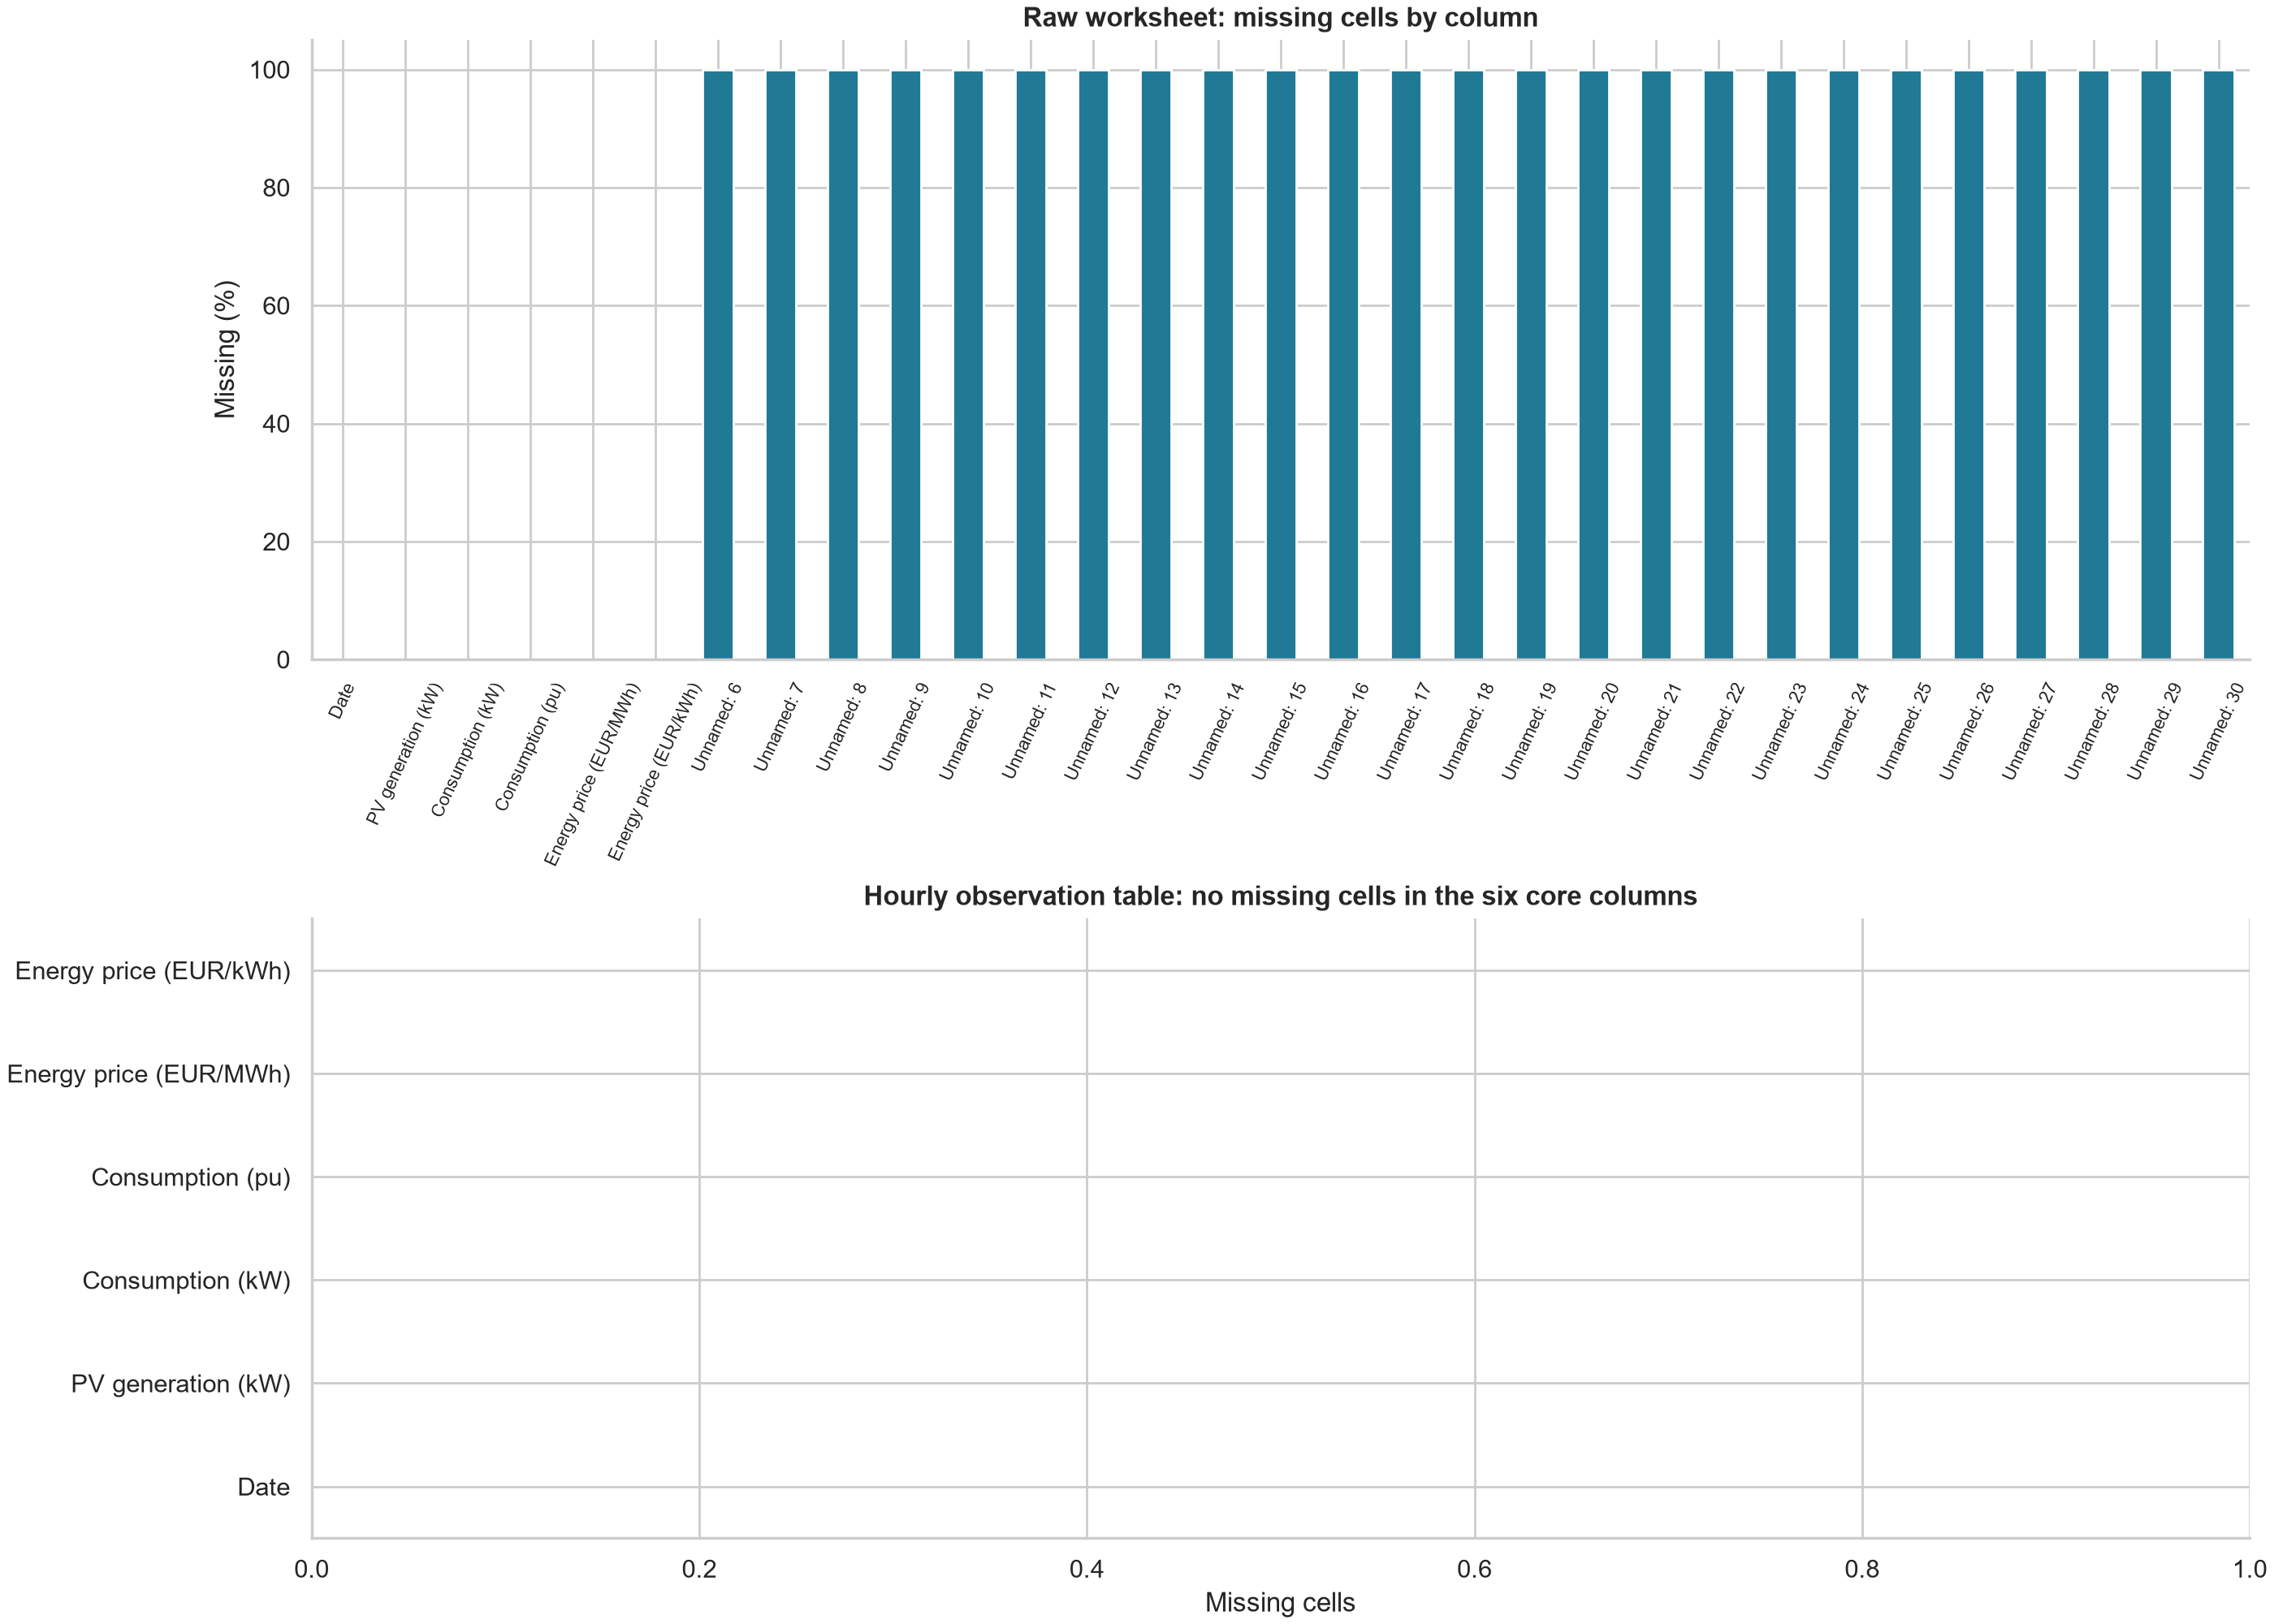
\includegraphics[width=0.95\linewidth]{figures/missing_values.png}
\caption{Missing value analysis distinguishing raw-sheet blank areas from complete core hourly table.}
\label{fig:missing_values}
\end{figure}

\begin{itemize}
    \item \textbf{Zero load}: 4 hours (2023-08-07 11:00–14:00), coincident with zero PV. Prices = 90 EUR/MWh throughout. Suggests shared outage or recording issue; not removed.
    \item \textbf{Zero price}: 70 hours in multiple runs; longest run 16 hours. Unit conversion verified; market validity unconfirmed.
    \item \textbf{Midday PV zeros}: 4 hours (same block as zero load), not additional events.
    \item \textbf{No missing timestamps, duplicates, or non-numeric values} in core hourly table.
\end{itemize}

All flags are documented in \texttt{outputs/step\_2/flagged\_values.csv} and \texttt{outputs/step\_3/suspicious\_values\_with\_context.csv} for downstream review.

\section{Conclusion}
\label{sec:conclusion}

This paper presented a comprehensive data mining analysis of a full-year hourly microgrid dataset (PV, load, price). The key results are:

\begin{enumerate}
    \item \textbf{Strong seasonal asymmetry}: Summer PV (1,184 kW mean) is 3.9$\times$ winter (307 kW), while winter load (2,919 kW) exceeds summer (2,161 kW) by 35\%. Summer prices are highest (95.8 EUR/MWh) despite high PV.
    \item \textbf{Correlation reversals under aggregation}: PV–Load shifts from +0.245 (hourly) to $-$0.292 (daily); PV–Price from $-$0.225 to +0.128. Modeling at a single time scale risks misleading conclusions.
    \item \textbf{Limited coincident solar utilization}: Only 23.8\% of demand is met by same-hour PV; 76.2\% requires grid import. Surplus occurs in just 8.8\% of hours.
    \item \textbf{Modest peak-price discount}: Top 5\% load hours average about 10 EUR/MWh below non-peak hours.
    \item \textbf{Data quality}: Four-hour coincident zero-load/zero-PV block and 70 zero-price hours flagged for source verification; no observations removed.
\end{enumerate}

\textbf{Practical implications:} Microgrid planners should (a) use season-specific profiles, not annual averages; (b) model hourly and daily correlations separately; (c) recognize that storage is essential to shift surplus to deficit hours; (d) validate zero-value events with the data provider before forecasting.

\textbf{Limitations:} Single year, single site, no weather data, no holiday classification, no storage or network constraints modeled. Timezone unknown—hour labels are workbook time.

\textbf{Future work:} (1) Multi-year data for climate trend robustness; (2) Battery scheduling optimization using the surplus/deficit profiles; (3) Deep learning forecasting (LSTM, Temporal Fusion Transformers) with seasonal features; (4) Scenario reduction via k-means clustering on daily profiles with silhouette/elbow validation; (5) Integration of weather forecasts for causal attribution.

\begin{thebibliography}{00}
\bibitem{b1} Mellit, A., \& Pavan, A. M., ``A 24-h forecast of solar irradiance using artificial neural networks: Application for performance prediction of a grid-connected PV plant,'' \textit{Renewable Energy}, vol. 35, no. 11, pp. 2511--2517, 2010.
\bibitem{b2} Voyant, C., et al., ``Machine learning methods for solar radiation forecasting: A review,'' \textit{Renewable and Sustainable Energy Reviews}, vol. 56, pp. 356--371, 2016.
\bibitem{b3} Hong, T., et al., ``Probabilistic energy forecasting: Global Energy Forecasting Competition 2014 and beyond,'' \textit{International Journal of Forecasting}, vol. 32, no. 3, pp. 896--913, 2016.
\bibitem{b4} Weron, R., ``Electricity price forecasting: A review of the state-of-the-art with a look into the future,'' \textit{International Journal of Forecasting}, vol. 30, no. 4, pp. 1030--1081, 2014.
\bibitem{b5} Heitsch, H., \& R\"omisch, W., ``Scenario reduction algorithms in stochastic programming,'' \textit{Computational Optimization and Applications}, vol. 24, pp. 187--206, 2003.
\bibitem{b6} Dupacov\'a, J., Gr\"owe-Kuska, N., \& R\"omisch, W., ``Scenario reduction in stochastic programming: An approach using probability metrics,'' \textit{Mathematical Programming}, vol. 95, pp. 493--511, 2003.
\bibitem{b7} Zhang, Y., et al., ``Clustering-based scenario generation for microgrid optimization,'' \textit{IEEE Transactions on Smart Grid}, vol. 10, no. 4, pp. 3892--3903, 2019.
\bibitem{b8} Liu, Z., et al., ``Correlation analysis of PV, load and price for microgrid energy management,'' \textit{Applied Energy}, vol. 250, pp. 112--124, 2019.
\bibitem{b9} Antonanzas, J., et al., ``Review of photovoltaic power forecasting,'' \textit{Solar Energy}, vol. 136, pp. 78--111, 2016.
\bibitem{b10} Deb, C., et al., ``A review on time series forecasting techniques for building energy consumption,'' \textit{Renewable and Sustainable Energy Reviews}, vol. 74, pp. 902--924, 2017.
\bibitem{b11} Lago, J., et al., ``Forecasting day-ahead electricity prices: A review of state-of-the-art algorithms, best practices and an open-access benchmark,'' \textit{Applied Energy}, vol. 293, p. 116983, 2021.
\bibitem{b12} Keane, A., et al., ``Scenario generation for stochastic optimization of renewable energy systems,'' \textit{IEEE Transactions on Power Systems}, vol. 30, no. 1, pp. 456--465, 2015.
\bibitem{b13} Pinson, P., et al., ``Scenario generation for stochastic programming: An application to wind energy,'' \textit{European Journal of Operational Research}, vol. 197, no. 3, pp. 1116--1125, 2009.
\bibitem{b14} Bessa, R. J., et al., ``Time series forecasting for renewable energy integration: A review,'' \textit{Wiley Interdisciplinary Reviews: Energy and Environment}, vol. 6, no. 1, p. e216, 2017.
\bibitem{b15} Chicco, G., et al., ``Data quality issues in smart meter data for energy analytics,'' \textit{IEEE Transactions on Smart Grid}, vol. 11, no. 4, pp. 3456--3467, 2020.
\bibitem{b16} Zhang, S., et al., ``Multi-variable clustering for scenario reduction in microgrid planning,'' \textit{Energy}, vol. 239, p. 122045, 2022.
\bibitem{b17} Ahmed, R., et al., ``A review on data-driven approaches for microgrid energy management,'' \textit{Renewable and Sustainable Energy Reviews}, vol. 154, p. 111823, 2022.
\bibitem{b18} Shahidehpour, M., et al., ``Data analytics for smart grids: Challenges and opportunities,'' \textit{Proceedings of the IEEE}, vol. 108, no. 9, pp. 1528--1545, 2020.
\bibitem{b19} Haben, S., et al., ``Review of low voltage load forecasting: Methods, applications, and recommendations,'' \textit{Applied Energy}, vol. 304, p. 117798, 2021.
\bibitem{b20} Ziel, F., et al., ``Day-ahead electricity price forecasting with high-dimensional structures: A review of recent advances,'' \textit{International Journal of Forecasting}, vol. 39, no. 1, pp. 130--154, 2023.
\end{thebibliography}

\end{document}